\documentclass[twoside]{article}
\usepackage{../estilo-ejercicios}
\usepackage{wasysym}
\usetikzlibrary{automata,positioning}
\usepackage{mathdots}
\usepackage{listings}
%--------------------------------------------------------
\begin{document}

\title{Ciencias de la Computación}

\author{Javier Aguilar Martín, Diego Pedraza López}
\maketitle

\begin{ejercicio}{1}
Para cada uno de los siguientes lenguajes sobre el alfabeto $\Sigma=\{a,b\}$, construye un autómata finito determinista que lo acepte. 
\begin{enumerate}
\item $L_1=\{w\in\Sigma^*:$ cada $a$ en $w$ está seguida o precedida por una $b\}$.
\item $L_2=\{w\in\Sigma^*: w$ contiene $abab$ como subpalabra $\}$.
\item $L_3= \{w\in\Sigma^*: w$ contiene un número par de $a$'s y un número impar de $b$'s$\}$.
\item $L_4= \{w\in\Sigma^*: w$ contiene $ab$ y $ba$ como subpalabras$\}$.
\end{enumerate}
\end{ejercicio}
\begin{solucion}\
\begin{enumerate}
\item 

\begin{figure}[h!]
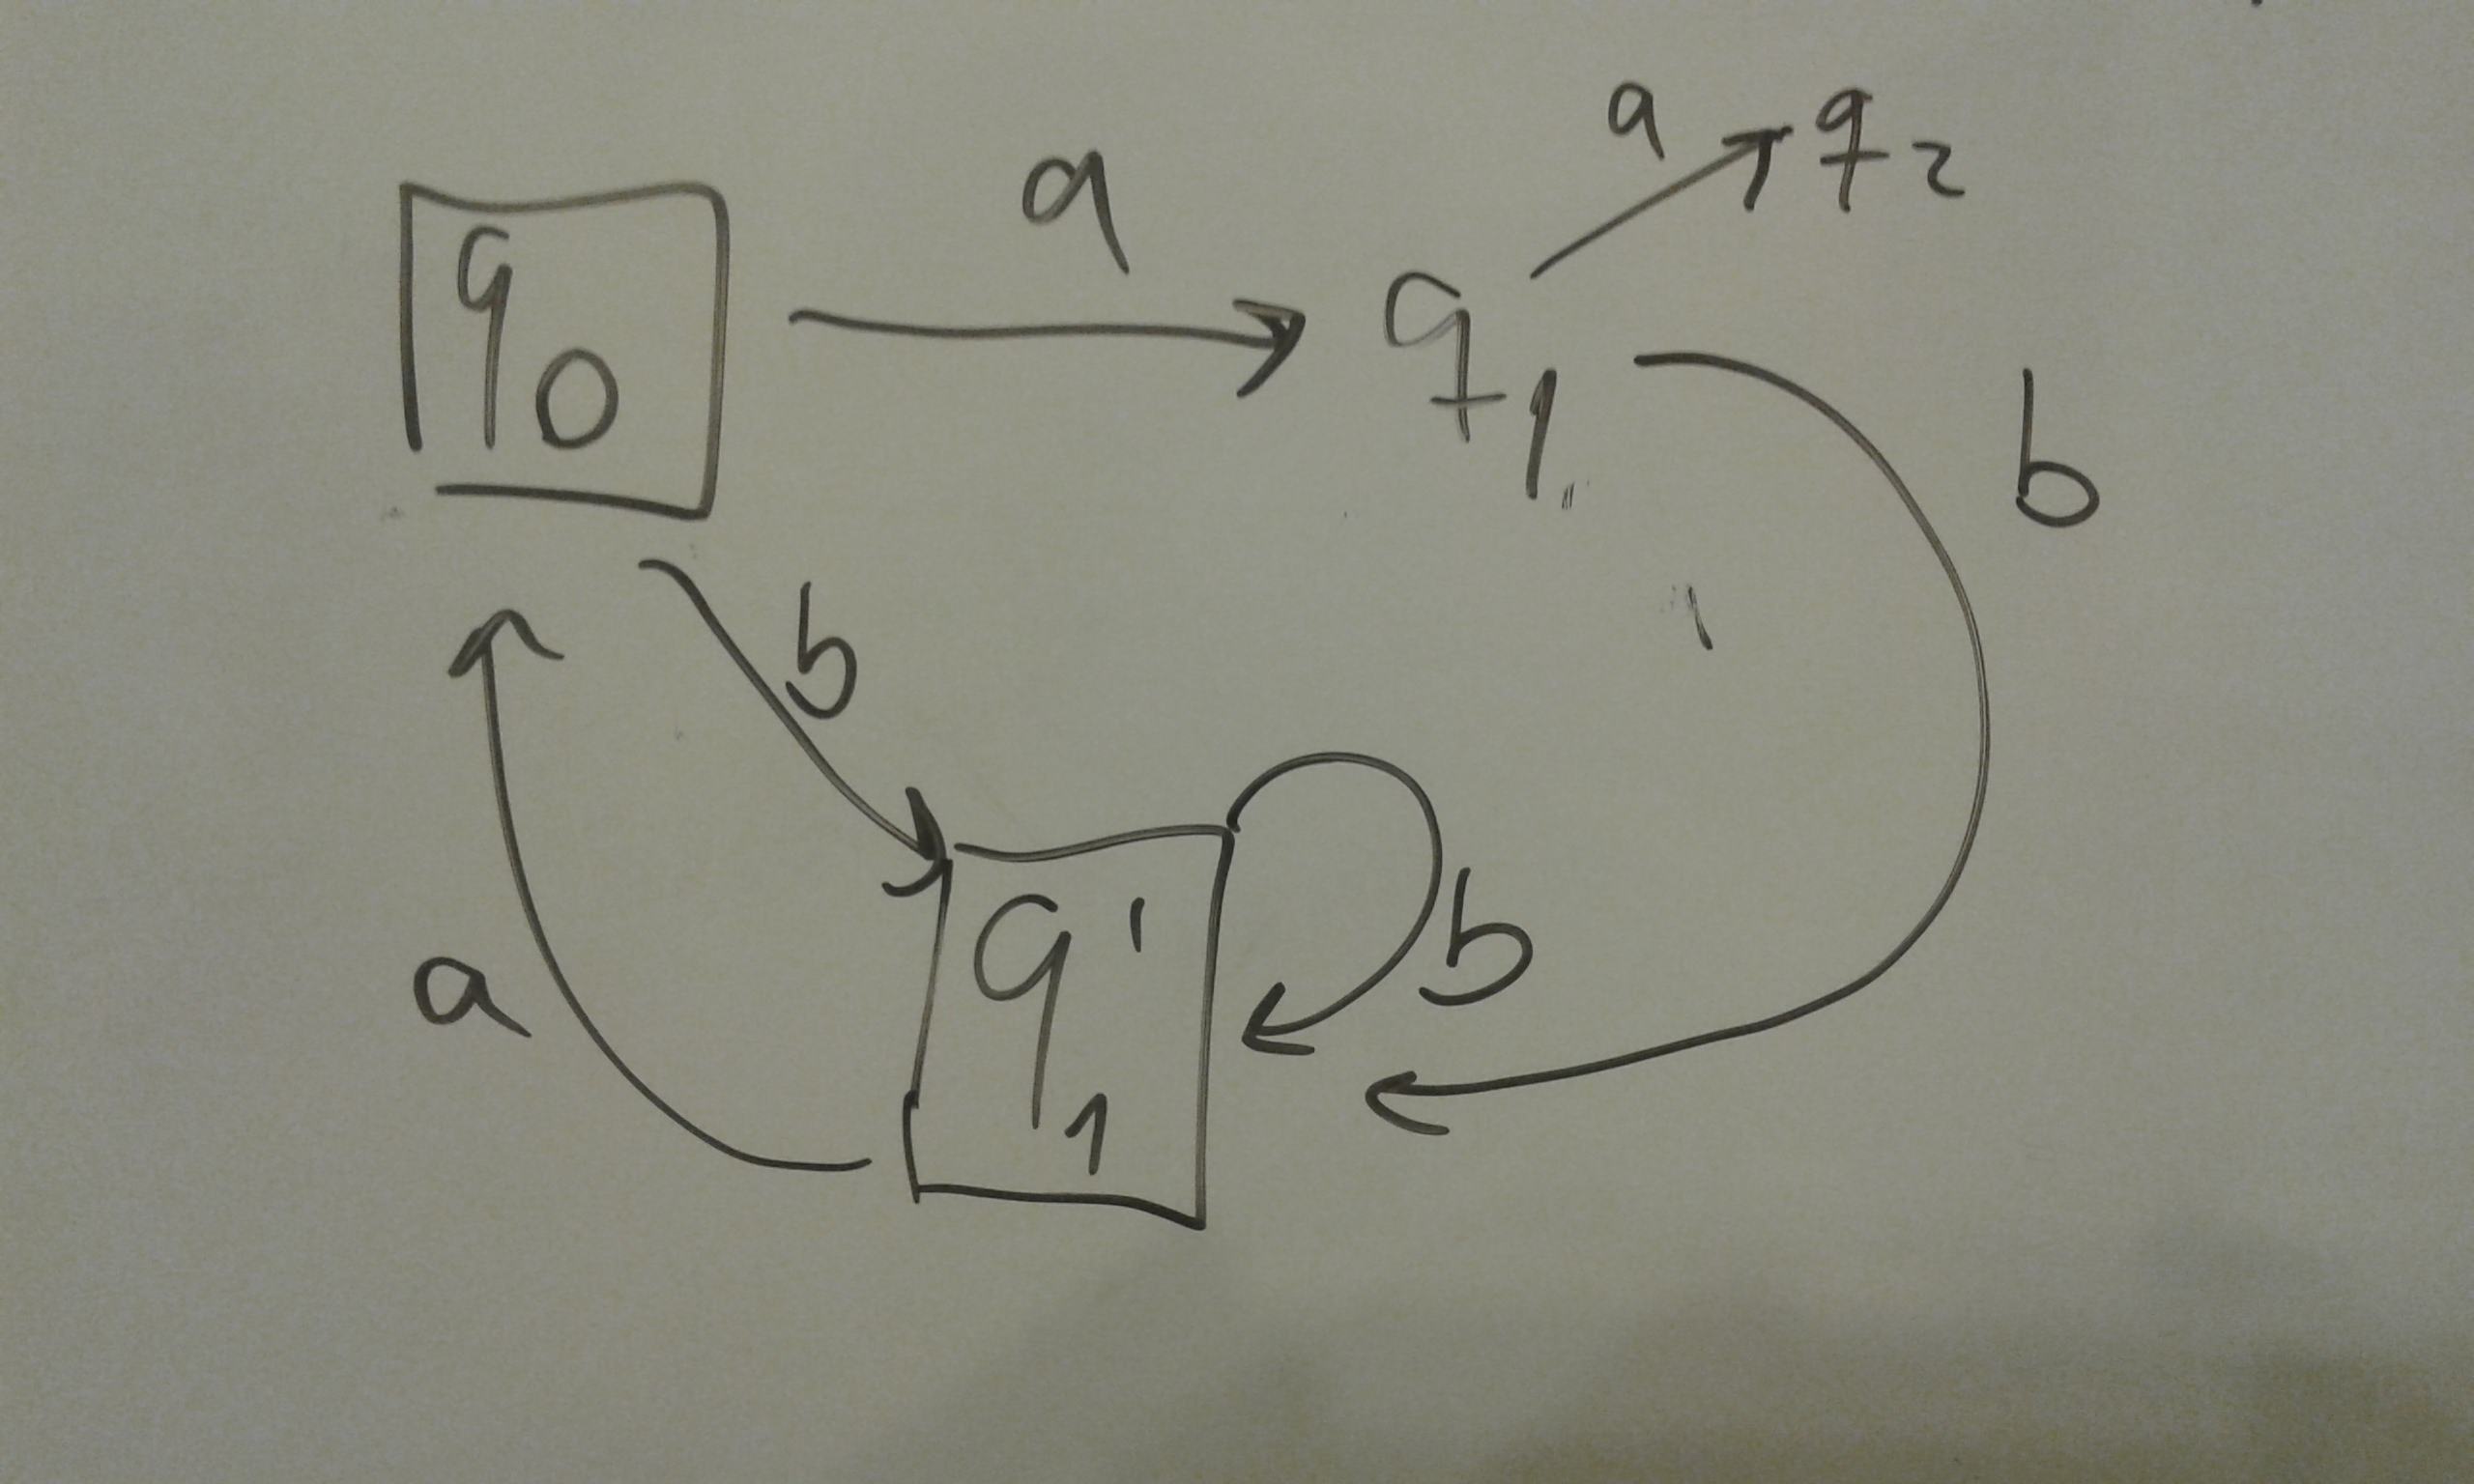
\includegraphics[scale=0.1]{Automatas/1-1}
\end{figure}\

\newpage

\item

 \begin{figure}[h!]
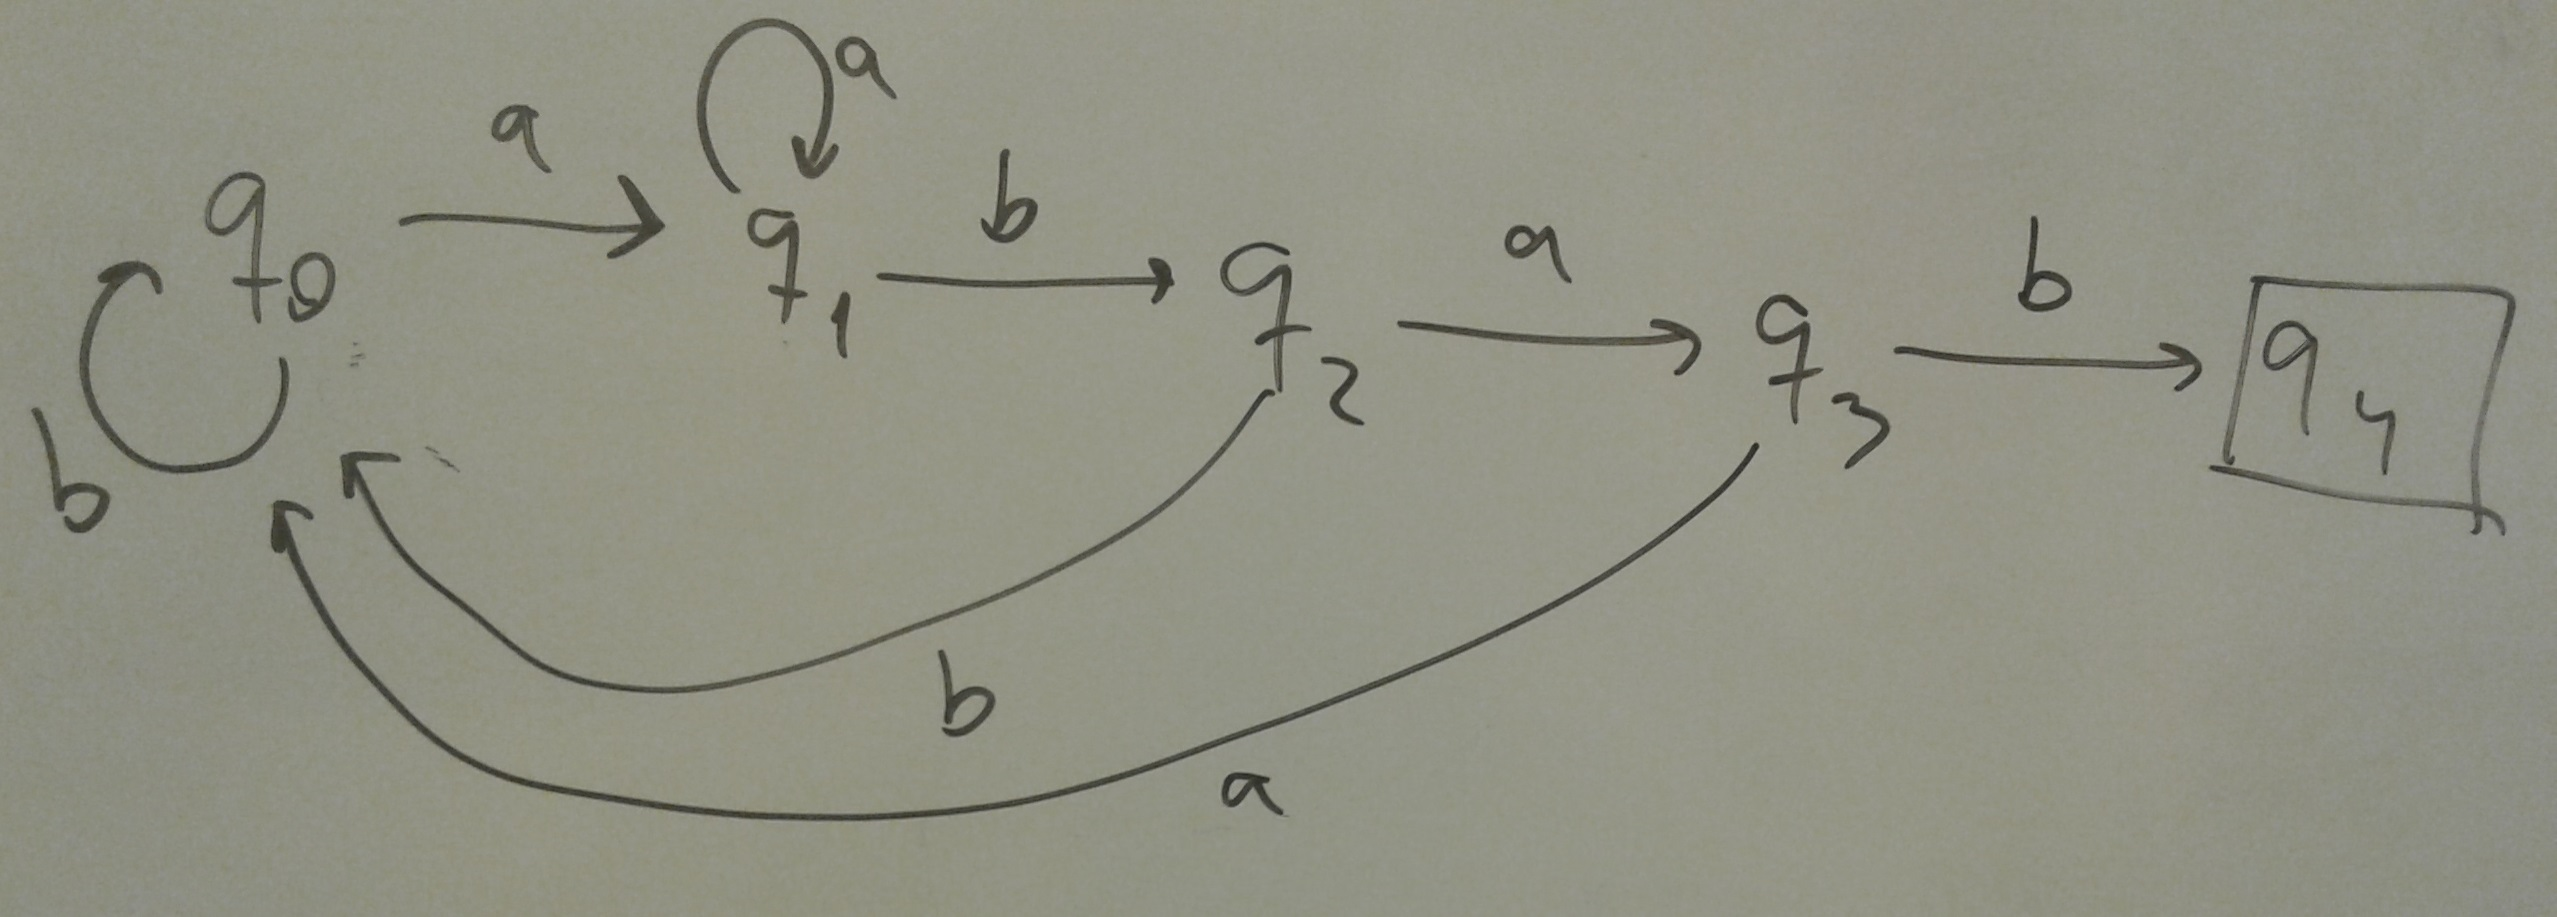
\includegraphics[scale=0.1]{Automatas/1-2}
\end{figure}\

\item 

\begin{figure}[h!]
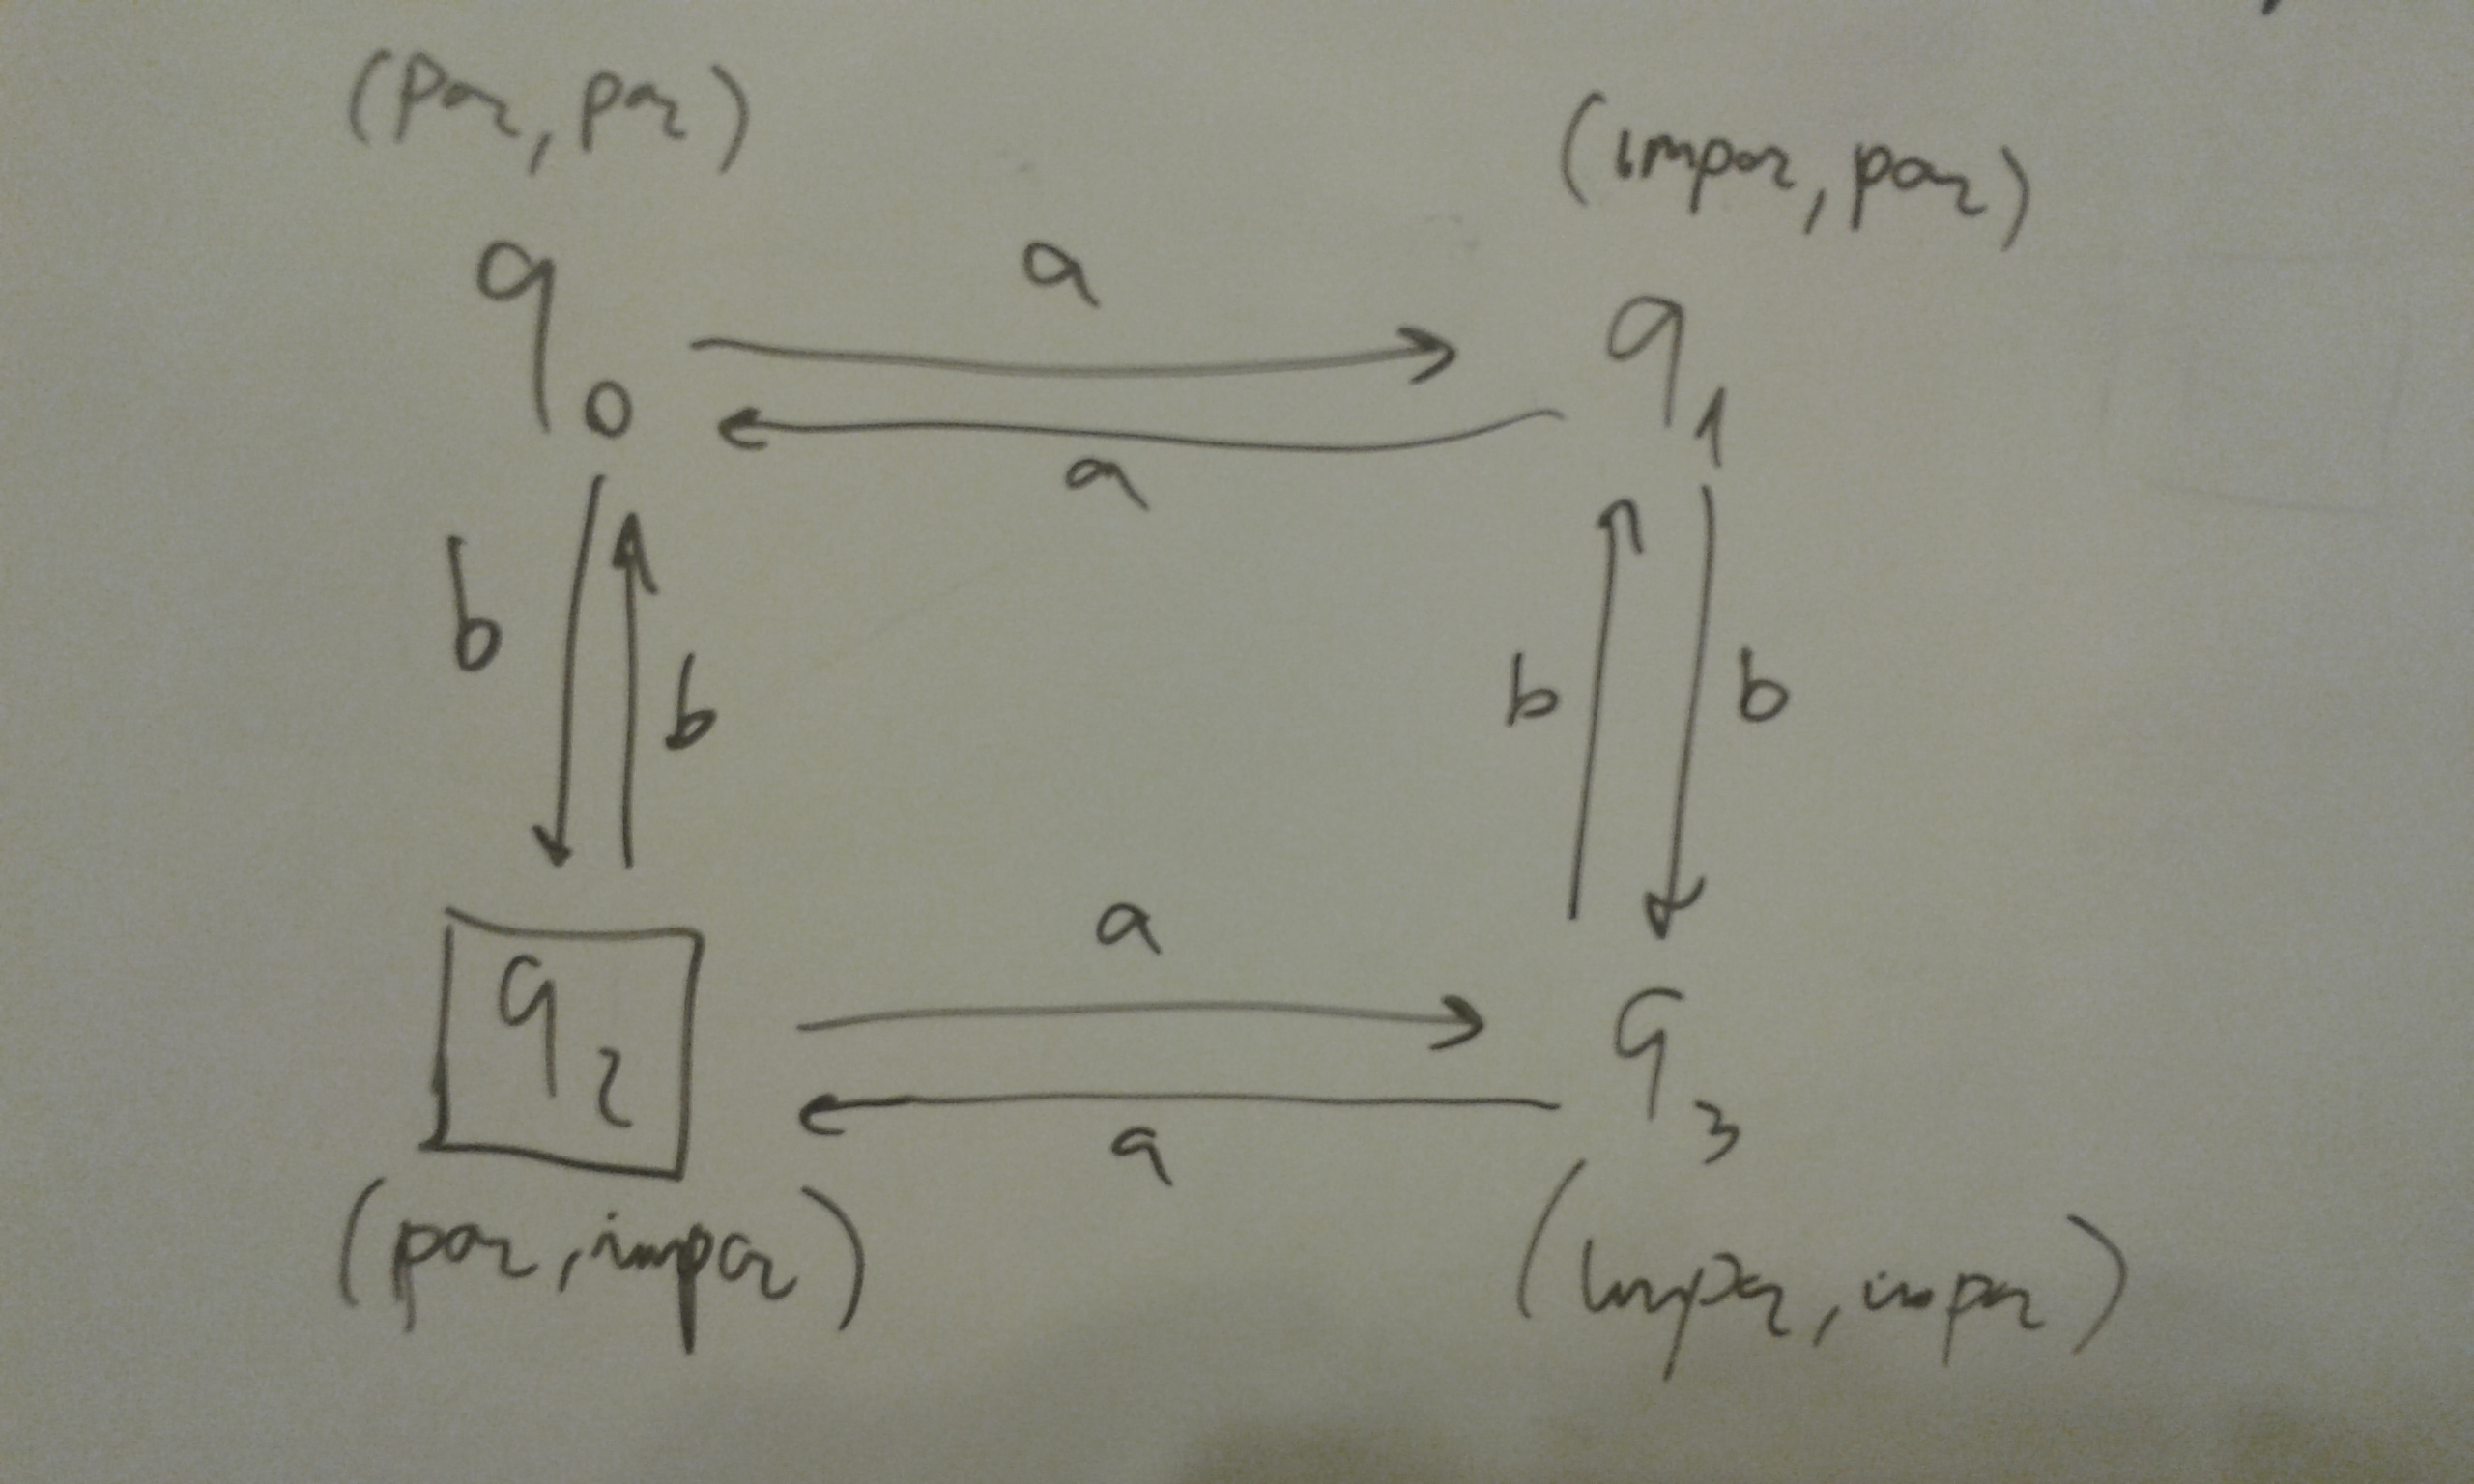
\includegraphics[scale=0.1]{Automatas/1-3}
\end{figure}\

\item 

\begin{figure}[h!]
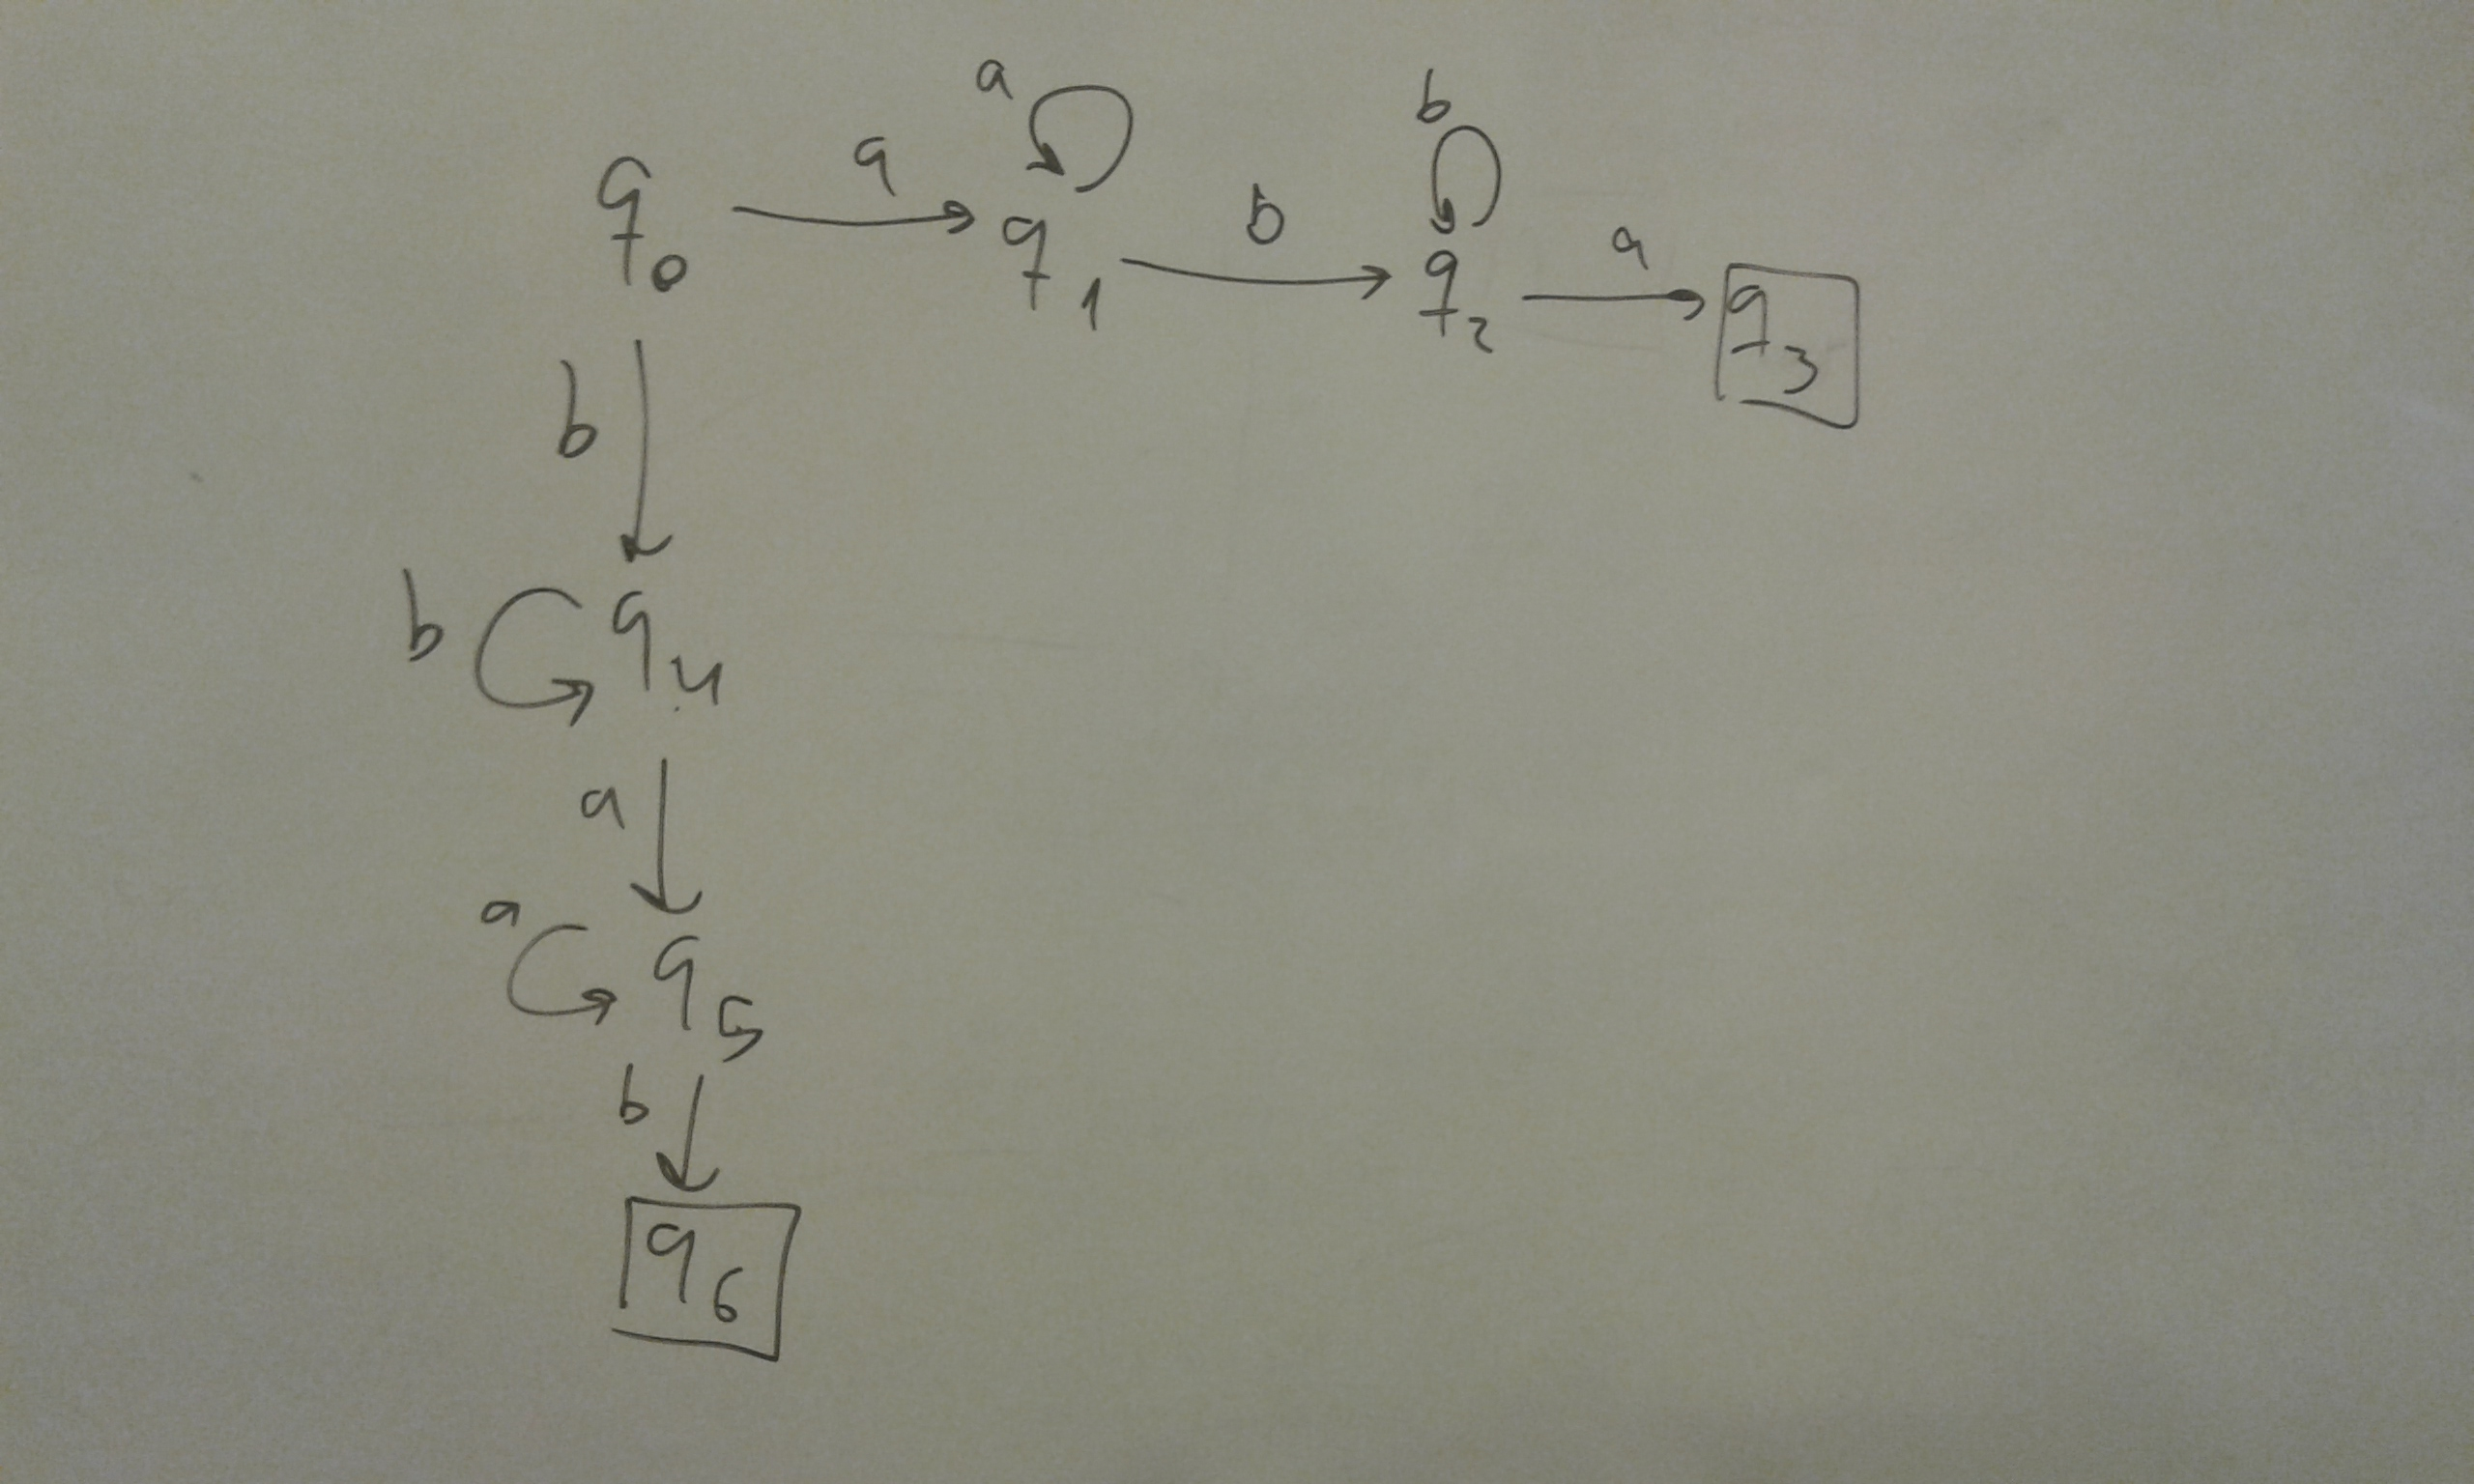
\includegraphics[scale=0.1]{Automatas/1-4}
\end{figure}\
\end{enumerate}
\end{solucion}

\newpage

\begin{ejercicio}{2}
Describe el lenguaje aceptado por cada uno de los siguientes autómatas

\begin{enumerate}
	\item[$M_1$:]
	\[
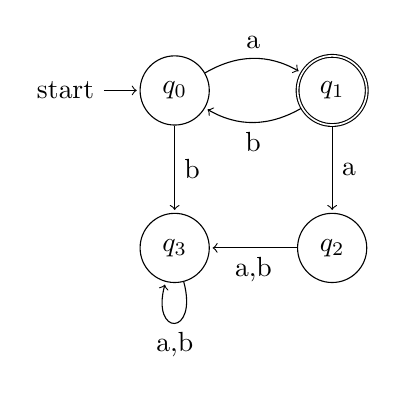
\begin{tikzpicture}[shorten >=1pt,node distance=2cm,on grid,auto] 
   \node[state,initial] (q_0)   {$q_0$}; 
   \node[state,accepting] (q_1) [right=of q_0] {$q_1$};
   \node[state] (q_2) [below=of q_1] {$q_2$};
   \node[state] (q_3) [below=of q_0] {$q_3$};
    \path[->] 
    (q_0) edge [bend left] node {a} (q_1)
          edge node {b} (q_3)
    (q_1) edge [bend left] node {b} (q_0)
          edge node {a} (q_2)
    (q_2) edge node {a,b} (q_3)
    (q_3) edge [loop below] node {a,b} ();
\end{tikzpicture}
\]

	\item[$M_2$:] 
	\[ 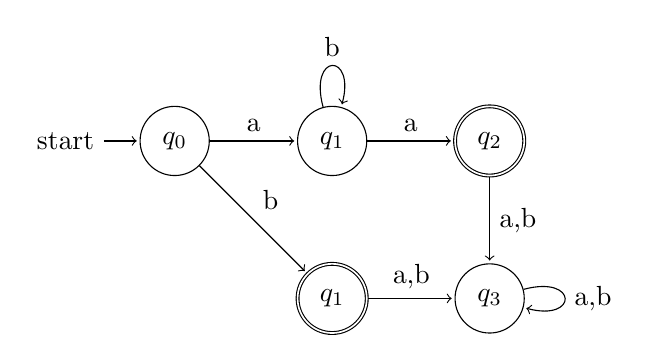
\begin{tikzpicture}[shorten >=1pt,node distance=2cm,on grid,auto] 
   \node[state,initial] (q_0)  {$q_0$}; 
   \node[state] (q_1) [right=of q_0] {$q_1$};
   \node[state,accepting] (q_2) [right=of q_1] {$q_2$};
   \node[state] (q_3) [below=of q_2] {$q_3$};
   \node[state,accepting] (q_4) [below=of q_1] {$q_1$};
    \path[->] 
    (q_0) edge node {a} (q_1)
          edge node {b} (q_4)
    (q_1) edge node {a} (q_2)
          edge [loop above] node {b} ()
    (q_2) edge node {a,b} (q_3)
    (q_3) edge [loop right] node {a,b} ()
    (q_4) edge node {a,b} (q_3);
\end{tikzpicture} \]

	\item[$M_3$:]
	\[ 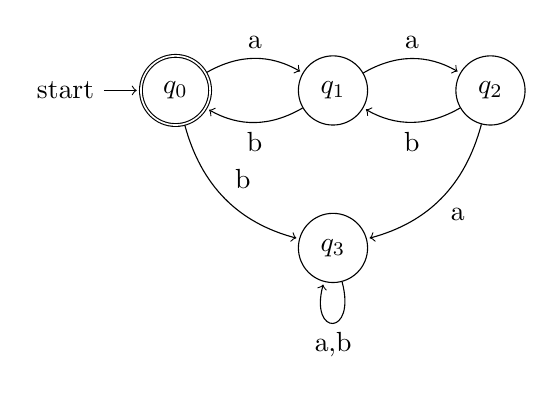
\begin{tikzpicture}[shorten >=1pt,node distance=2cm,on grid,auto] 
   \node[state,initial,accepting] (q_0)  {$q_0$}; 
   \node[state] (q_1) [right=of q_0] {$q_1$};
   \node[state] (q_2) [right=of q_1] {$q_2$};
   \node[state] (q_3) [below=of q_1] {$q_3$};
    \path[->] 
    (q_0) edge [bend left] node {a} (q_1)
          edge [bend right] node {b} (q_3)
    (q_1) edge [bend left] node {b} (q_0)
          edge [bend left] node {a} (q_2)
    (q_2) edge [bend left] node {b} (q_1)
          edge [bend left] node {a} (q_3)
    (q_3) edge [loop below] node {a,b} ();
\end{tikzpicture} \]

	\item[$M_4$:]
	\[ 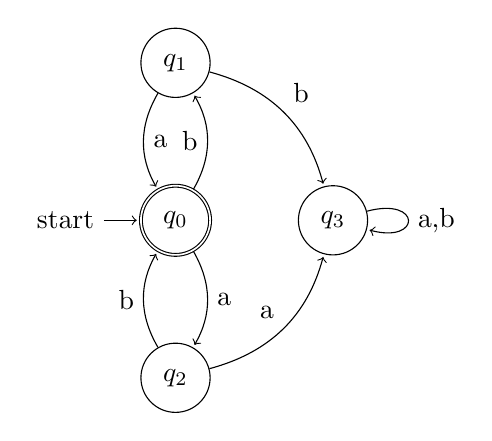
\begin{tikzpicture}[shorten >=1pt,node distance=2cm,on grid,auto] 
   \node[state,initial,accepting] (q_0)  {$q_0$}; 
   \node[state] (q_1) [above=of q_0] {$q_1$};
   \node[state] (q_2) [below=of q_0] {$q_2$};
   \node[state] (q_3) [right=of q_0] {$q_3$};
    \path[->] 
    (q_0) edge [bend right] node {b} (q_1)
          edge [bend left] node {a} (q_2)
    (q_1) edge [bend right] node {a} (q_0)
          edge [bend left] node {b} (q_3)
    (q_2) edge [bend left] node {b} (q_0)
          edge [bend right] node {a} (q_3)
    (q_3) edge [loop right] node {a,b} ();
\end{tikzpicture} \]
\end{enumerate}

\end{ejercicio}
\begin{solucion}\
\begin{enumerate}
\item $M_1$  acepta lo mismo que si quitamos la parte de abajo. Acepta el lenguaje $L(a(ba)^*)$.
\item Como tiene dos estados finales, el lenguaje aceptado es la únión de los lenguajes aceptados por los autómatas que solo tienen uno de los estados finales. Empecemos por $M_{2,1}$ que solo tiene $q_2$ como estado final. Nos podemos quedar con las palabras aceptadas por la parte superior del diagrama. $L(M_{2,1})=L(ab^*a)$. En $M_{2,2}$, pasa lo mismo, así que $L(M_{2,2})=L(b)=\underline{b}$. Por tanto, $L(M_1)=L(a(ba)^*)+\underline{b}=L(a(ba)^*+b)$.

Vamos a resolverlo también aplicando el método de la diapositiva 26.

\item Podemos eliminar cualquier cosa que vaya a $q_3$. $L(M_3)=L(a(ab)^*b)$. 

\item Podemos eliminar cualquier cosa que vaya a $q_3$. $L(M_4)=L((ba+ab)^*)$
\end{enumerate}
\end{solucion}

\newpage

\begin{ejercicio}{3}
¿Cuáles de las siguientes palabras son aceptadas por el siguiente $\varepsilon$-AFND?
\[ \begin{tikzpicture}[shorten >=1pt,node distance=2cm,on grid,auto] 
   \node[state,initial,accepting] (q_0)  {$q_0$}; 
   \node[state] (q_1) [right=of q_0] {$q_1$};
   \node[state] (q_2) [right=of q_1] {$q_2$};
   \node[state] (q_3) [right=of q_2] {$q_3$};
   \node[state] (q_4) [below=of q_1] {$q_4$};
   \node[state] (q_5) [left=of q_4] {$q_5$};
    \path[->] 
    (q_0) edge node {a} (q_1)
    (q_1) edge node {b} (q_2)
          edge node {ϵ} (q_4)
    (q_2) edge node {a} (q_3)
          edge [bend left] node {b} (q_4)
    (q_4) edge node {b} (q_0)
          edge node {b} (q_5)
    (q_5) edge node {a} (q_0);
\end{tikzpicture} \]

\begin{enumerate}
	\item $aa$.
	\item $aba$.
	\item $abb$.
	\item $abab$.
\end{enumerate}
\end{ejercicio}
\begin{solucion}\
\begin{enumerate}
\item No.
\item Sí, $q_0,q_1,q_4,q_5,q_0$.
\item No, si llegas a $q_0$ con $b$, $\hat{\delta}(q_0,b)=\varepsilon-cl(\emptyset)=\emptyset$, así que no cuenta porque no tiene salida. De hecho no puedes leer la letra y te quedas bloqueado.
\item Sí, $q_0,q_1,q_4,q_0,q_1,q_4$.
\end{enumerate}
\end{solucion}

\newpage

\begin{ejercicio}{6}
Para cada una de las siguientes expresiones regulares construir un $\varepsilon$-AFND que
acepte el lenguaje generado por ella:
\begin{enumerate}
\item $(ab)^*(ba)^*+aa^*$.
\item $((ab+aab)^*a^*)^*$.
\item $((a^*b+a^*)^*b)^*$.
\item $(ba + b)^* + (bb + a)^*$.
\end{enumerate}
\end{ejercicio}
\begin{solucion}\
\begin{enumerate}
\item El estado inicial debe ser final para aceptar la palabra vacía.

\begin{figure}[h!]
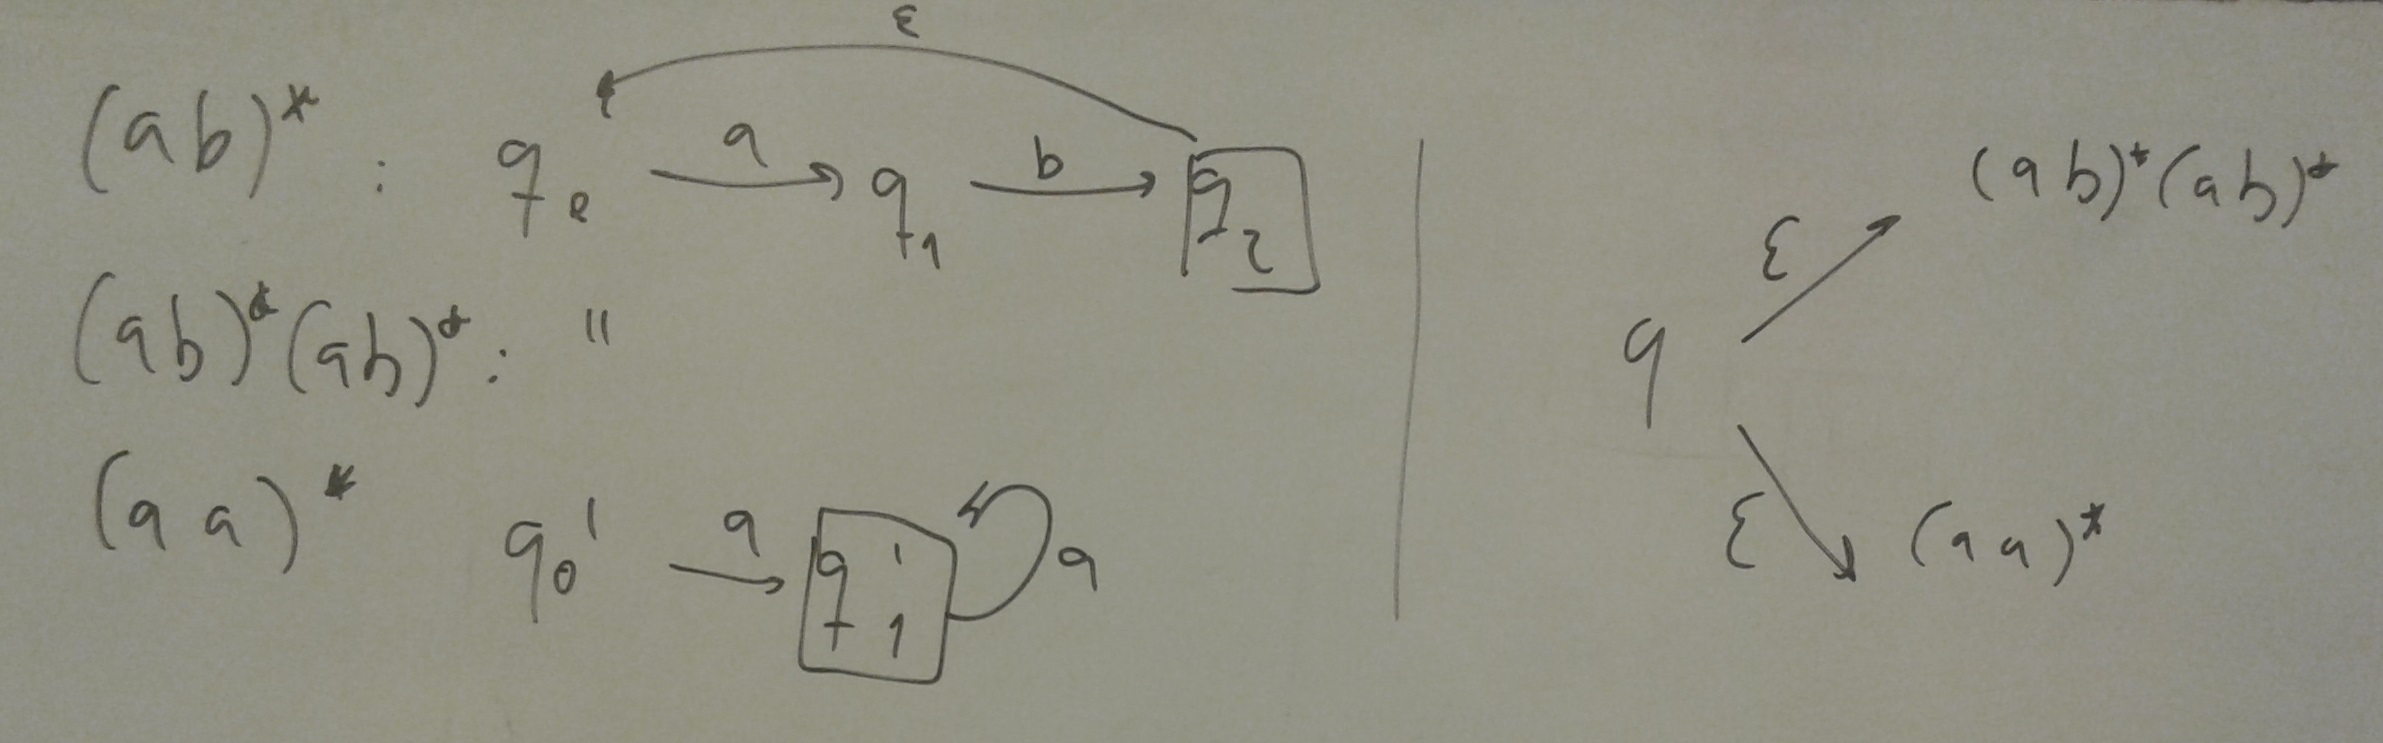
\includegraphics[scale=0.1]{Automatas/6-1}
\end{figure}\

\item 

\begin{figure}[h!]
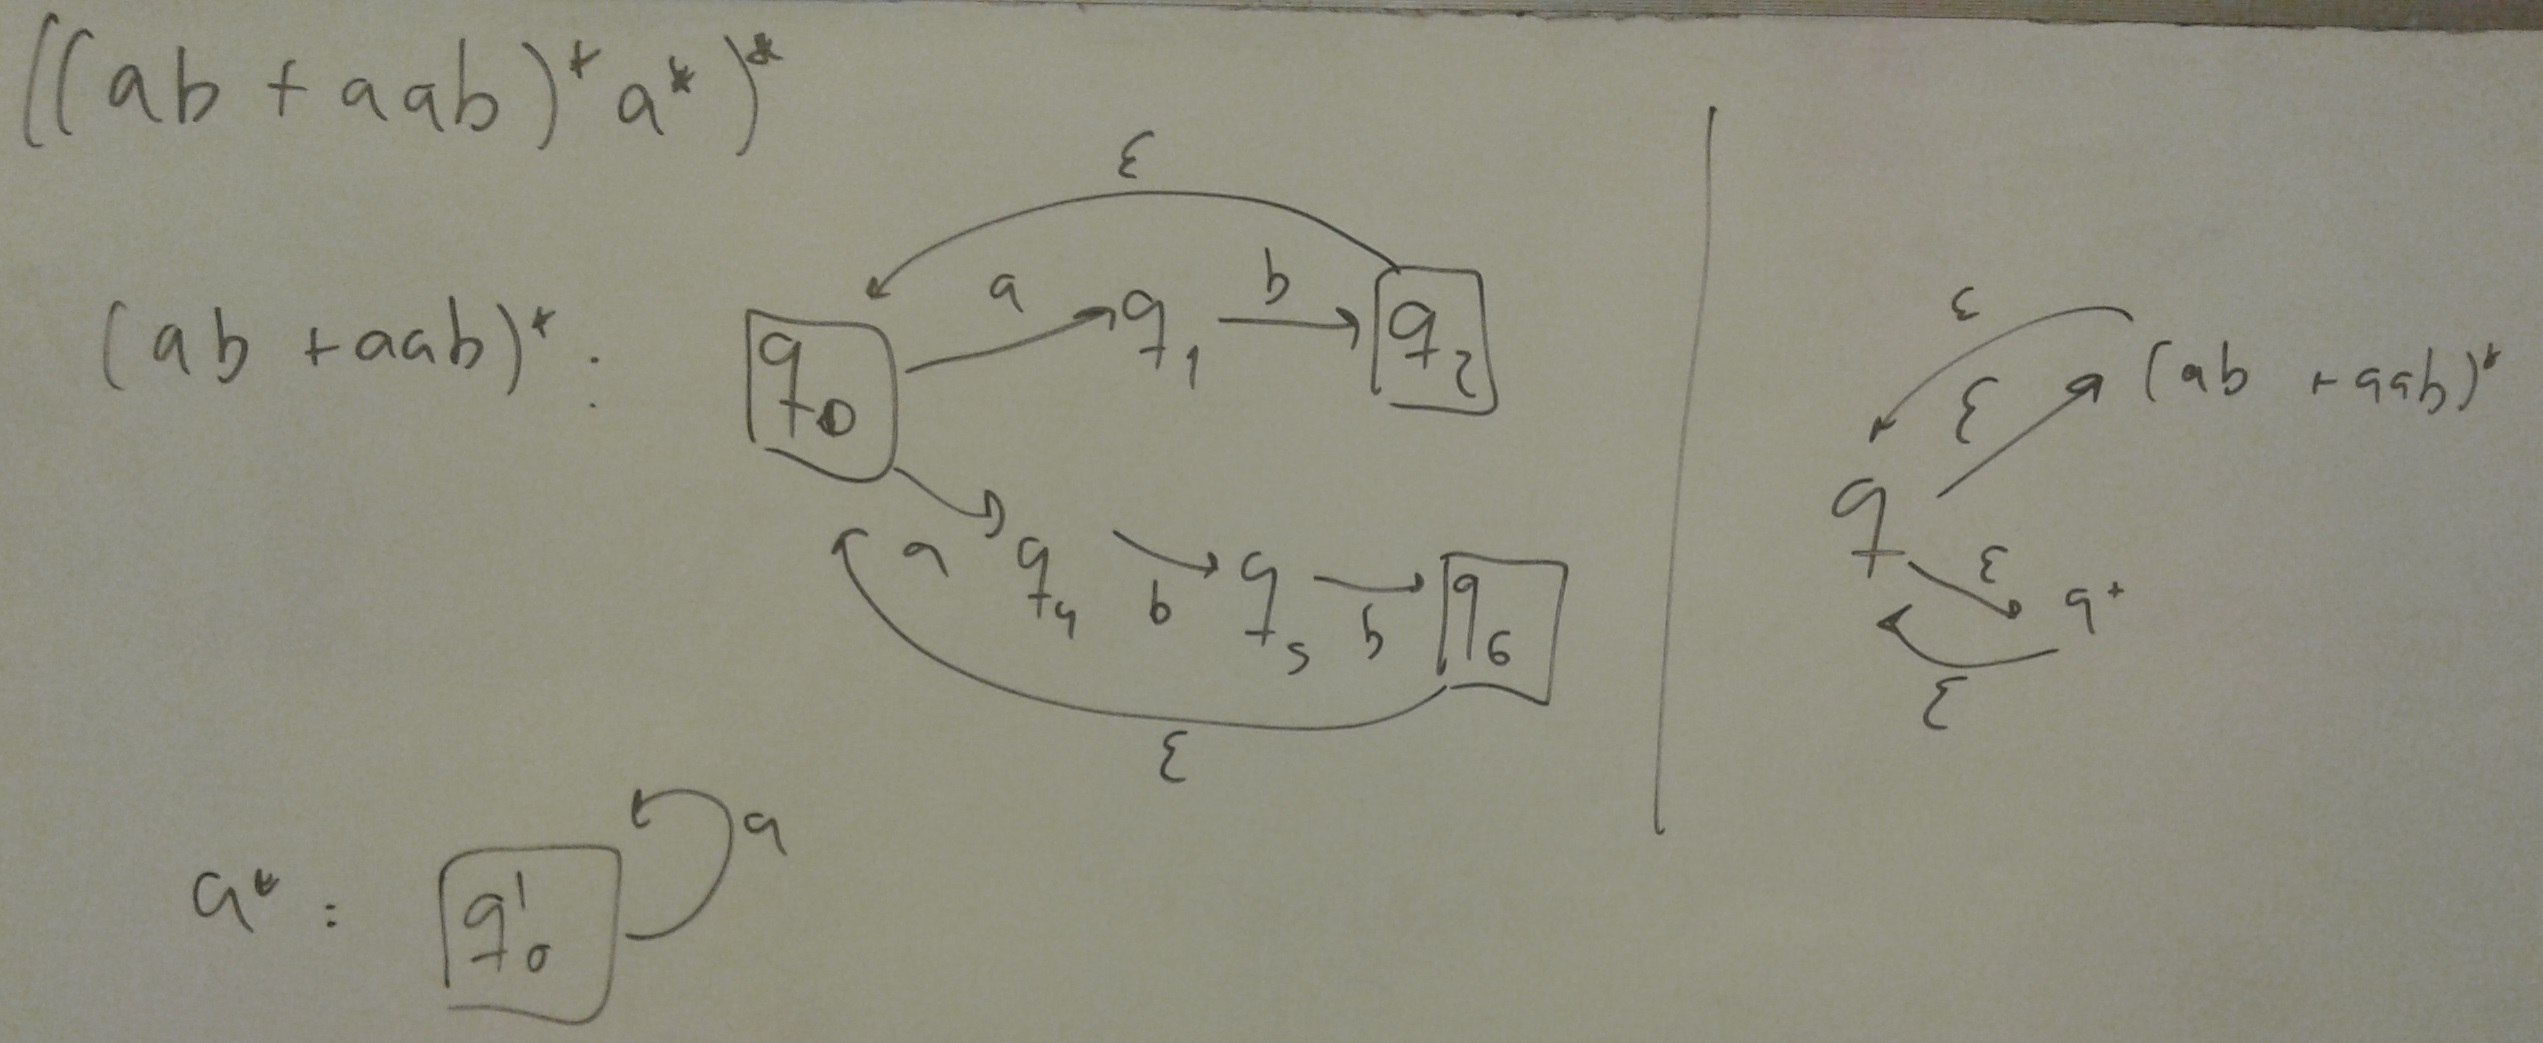
\includegraphics[scale=0.1]{Automatas/6-2}
\end{figure}\
\item

\begin{figure}[h!]
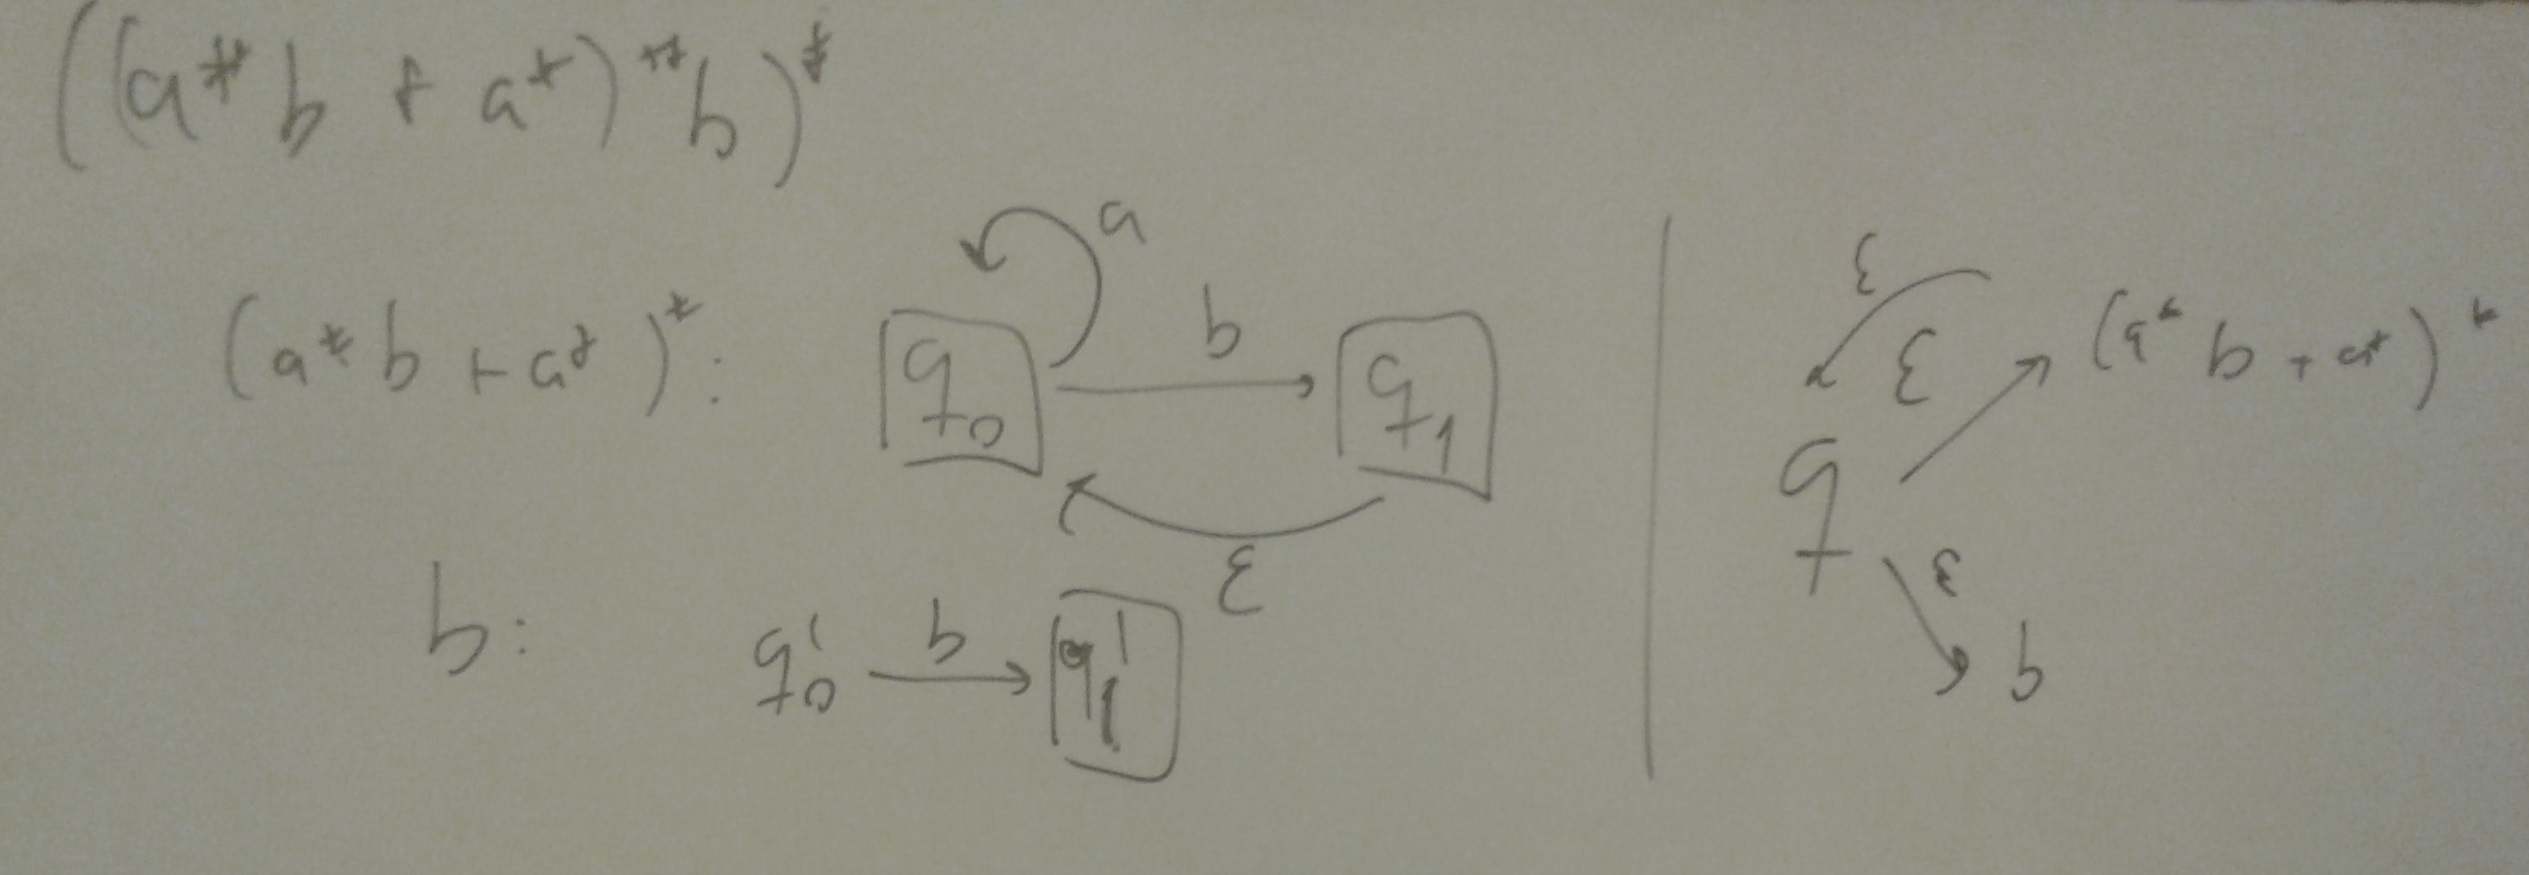
\includegraphics[scale=0.1]{Automatas/6-3}
\end{figure}\

\newpage

\item

\begin{figure}[h!]
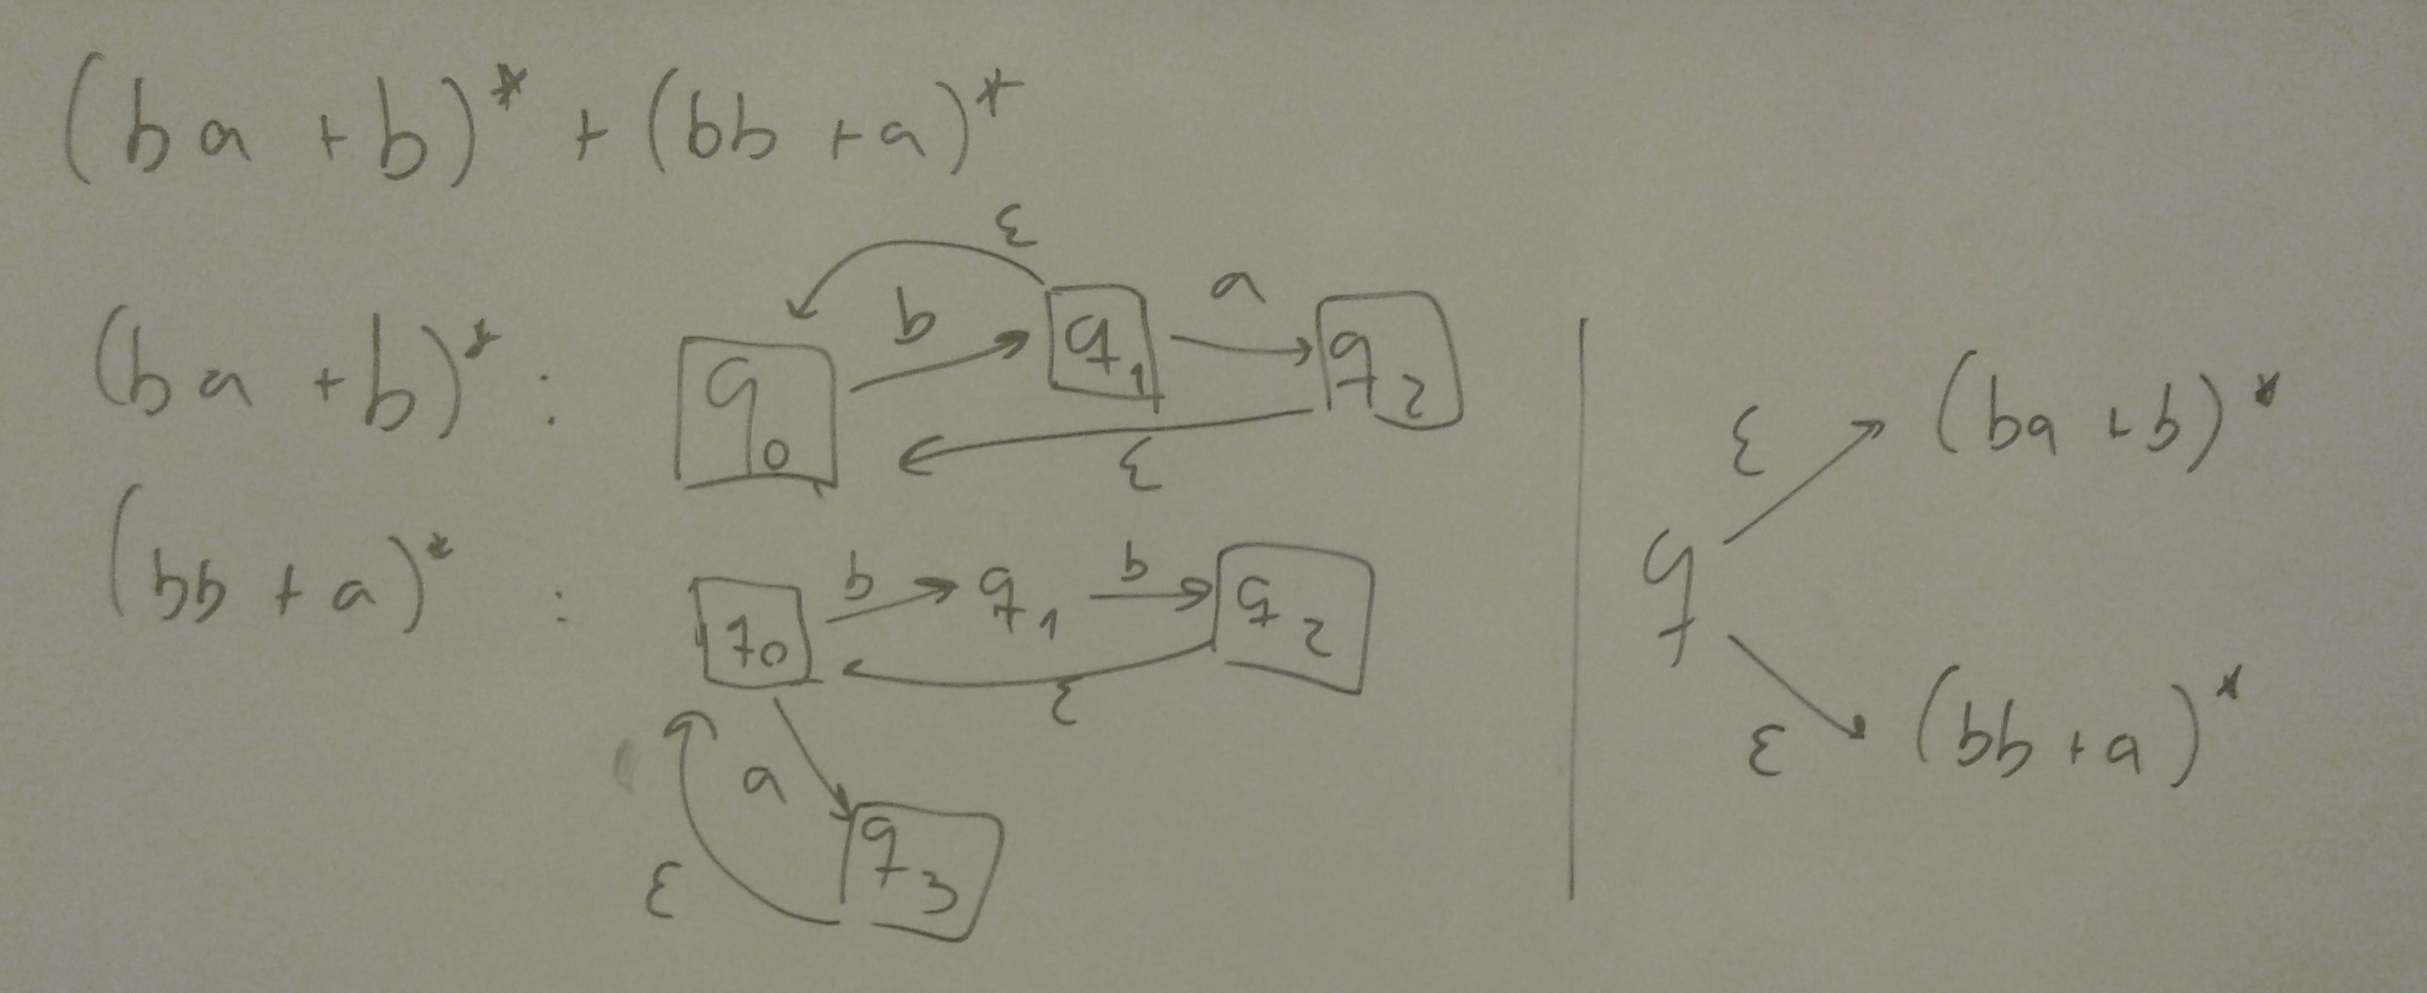
\includegraphics[scale=0.1]{Automatas/6-4}
\end{figure}\ 
\end{enumerate}
\end{solucion}

\newpage

\begin{ejercicio}{7}
Sea $L = L(((aa) + (aaa))^*)$. Encontrar un AFD que acepte $L$.
\end{ejercicio}
\begin{solucion}\

\begin{figure}[h!]
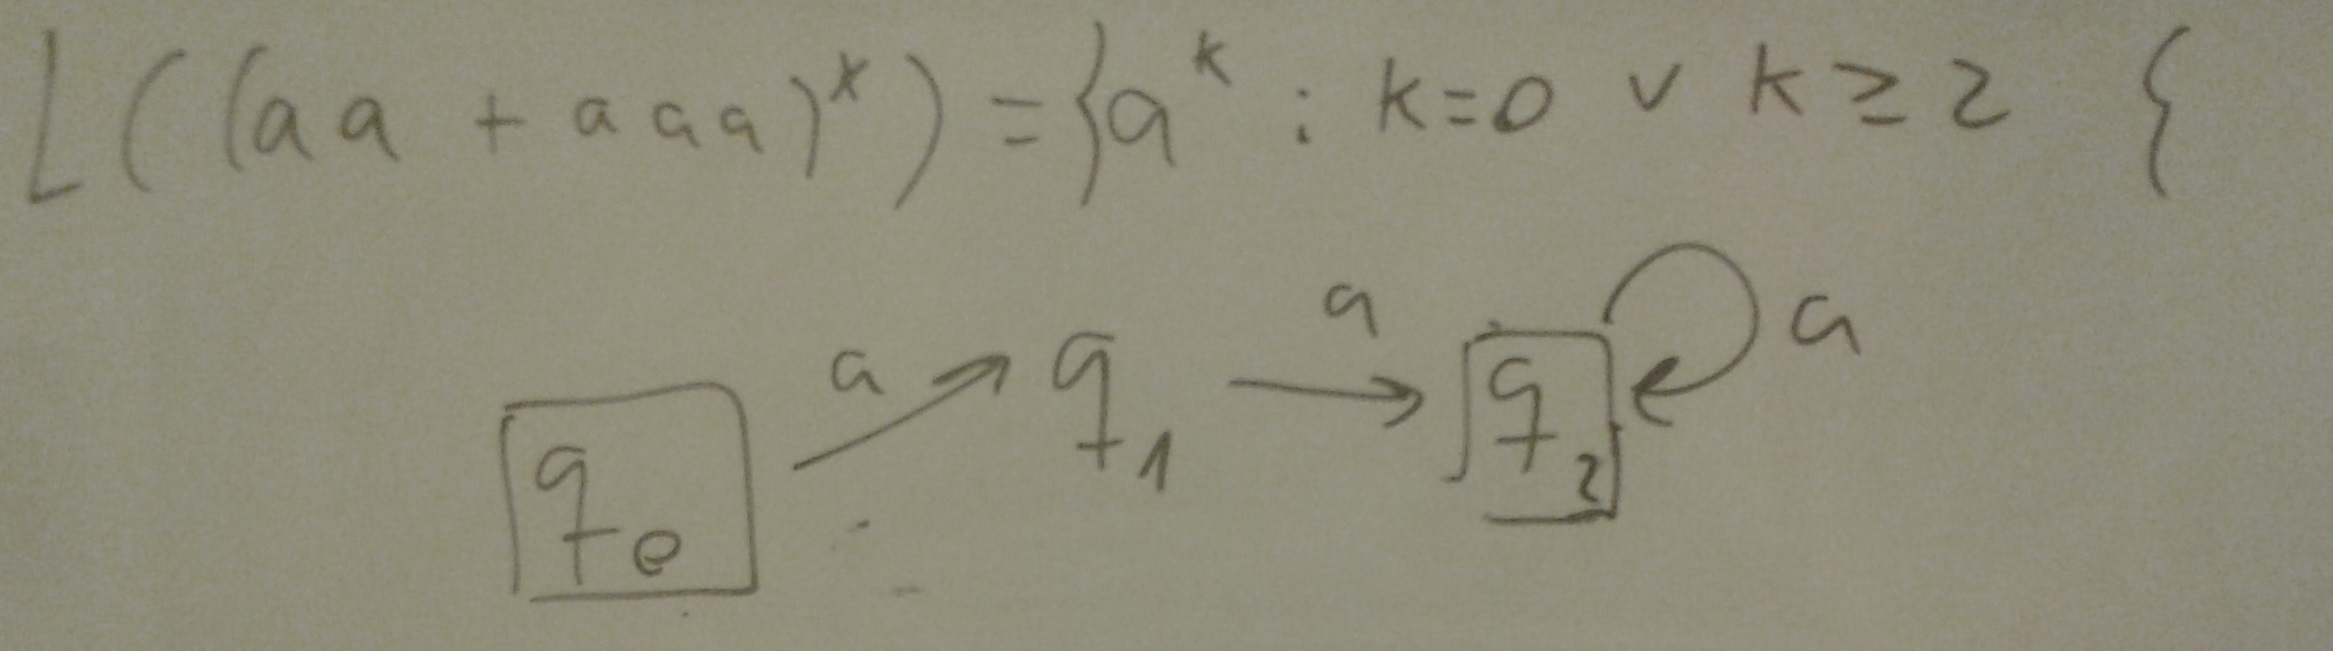
\includegraphics[scale=0.2]{Automatas/7}
\end{figure}\
\end{solucion}

\newpage

\begin{ejercicio}{8}
Condieremos el alfabeto
$$\Sigma_3 = \left\{\begin{bmatrix}
0\\
0\\
0
\end{bmatrix},\begin{bmatrix}
1\\
0\\
0
\end{bmatrix},\begin{bmatrix}
0\\
1\\
0
\end{bmatrix},\dots,\begin{bmatrix}
1\\
1\\
1
\end{bmatrix}\right\}$$

formado por todas la columnas de 0's y 1's de altura 3. Una palabra sobre $\Sigma_3$ puede identificarse
con una matriz de 3 filas formada por 0's y 1's, cada una de las cuales puede considerarse un
número natural en notación binaria. Probar que el lenguaje
$$B = \{w \in \Sigma^*_3: \text{la fila inferior es la suma de las dos filas superiores}\}$$
es regular.
\end{ejercicio}
\begin{solucion}
Hay que pensarlo con cuidao. Cada columna se corresponde a las columnas de una suma de números binarios. El autómata comprueba si la suma está bien hecha. Ojo con las llevadas. El autómata lee de izquiera a derecha así que hay que invertir los números. 
\end{solucion}
\newpage

\begin{ejercicio}{9}
Condieremos el alfabeto
$$\Sigma_2 = \left\{\begin{bmatrix}
0\\
0\\
\end{bmatrix},\begin{bmatrix}
1\\
0\\
\end{bmatrix},\begin{bmatrix}
0\\
1\\
\end{bmatrix},\begin{bmatrix}
1\\
1\\
\end{bmatrix}\right\}$$
formado por todas la columnas de 0's y 1's de altura 2. Una palabra sobre $\Sigma_2$ puede identificarse
con una matriz de 2 filas formada por 0's y 1's, cada una de las cuales puede considerarse un
número natural en notación binaria. Probar que los siguientes lenguajes son regulares:
\begin{enumerate}
\item $C = \{w \in \Sigma^*_2
: \text{la fila inferior es la superior multiplicada por } 3\}$. 
\item $D = \{w \in \Sigma^*_2
: \text{la fila inferior es menor que la superior}\}$.  
\end{enumerate}
\end{ejercicio}
\begin{solucion}


\begin{figure}[h!]
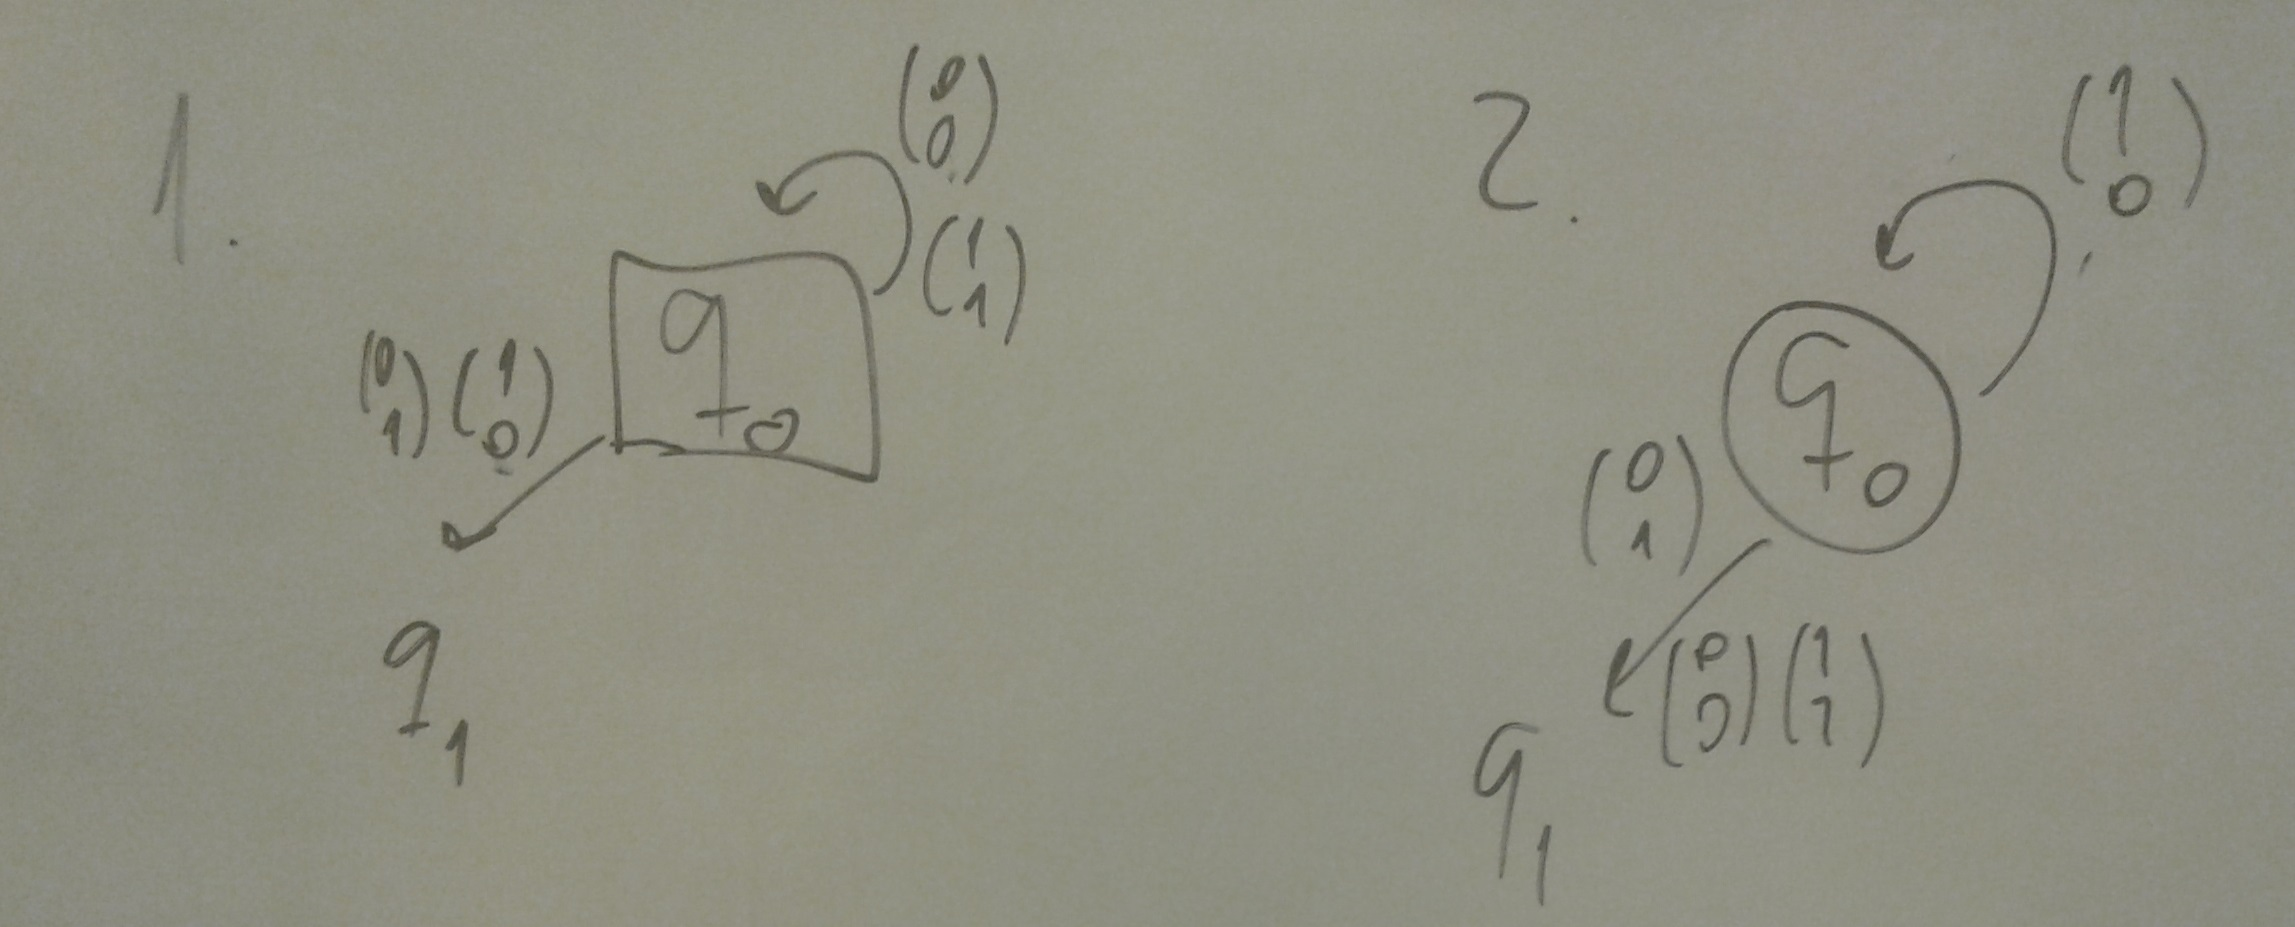
\includegraphics[scale=0.1]{Automatas/9}
\end{figure}\
\end{solucion}
\newpage

\begin{ejercicio}{11}
Construir un AFD equivalente al siguiente AFND:
\end{ejercicio}
\begin{solucion}\

\begin{figure}[h!]
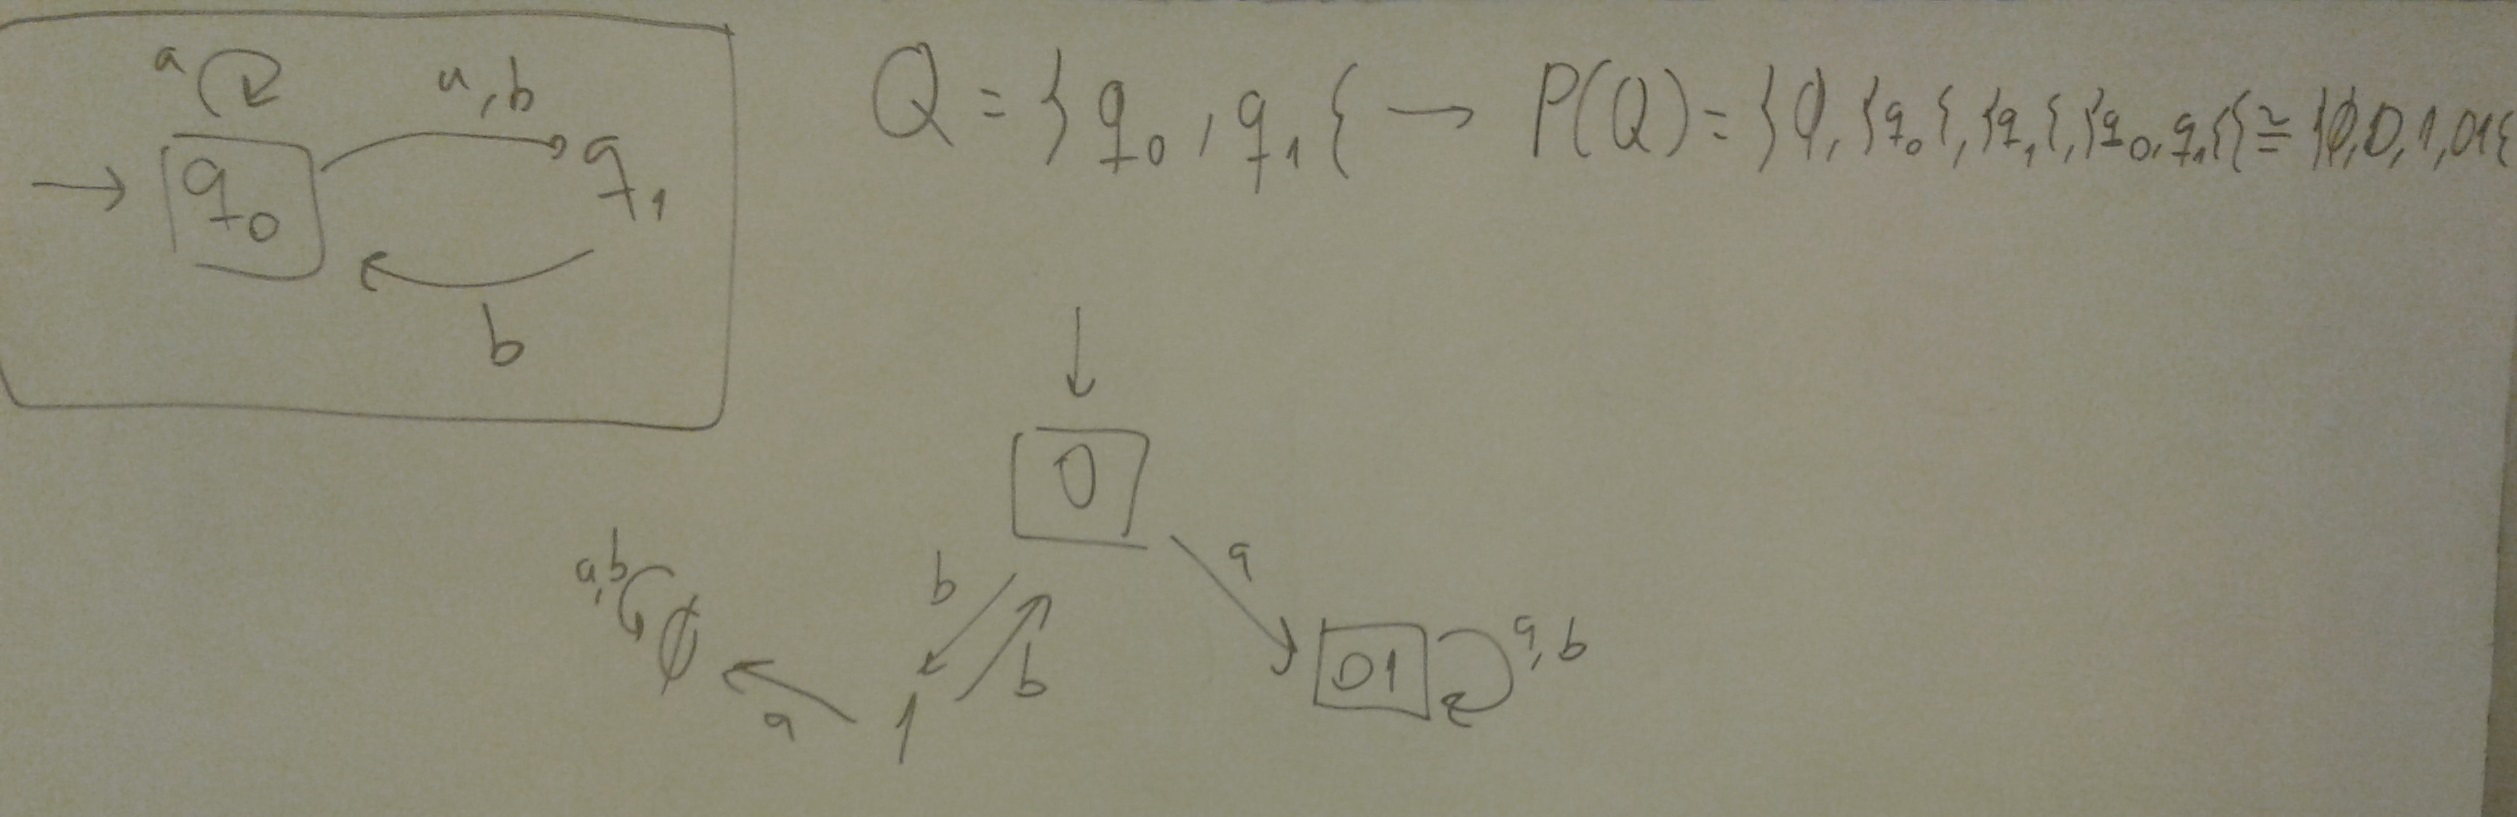
\includegraphics[scale=0.2]{Automatas/11}
\end{figure}\
\end{solucion}

\newpage

\begin{ejercicio}{12}
Construir un AFD equivalente al siguiente $\varepsilon$-AFND:
\end{ejercicio}
\begin{solucion}
Tener en cuenta que hay que hacer el $\varepsilon-$cl, es decir, ver si se puede llegar a algún sitio con un $\varepsilon$-movimiento.

\begin{figure}[h!]
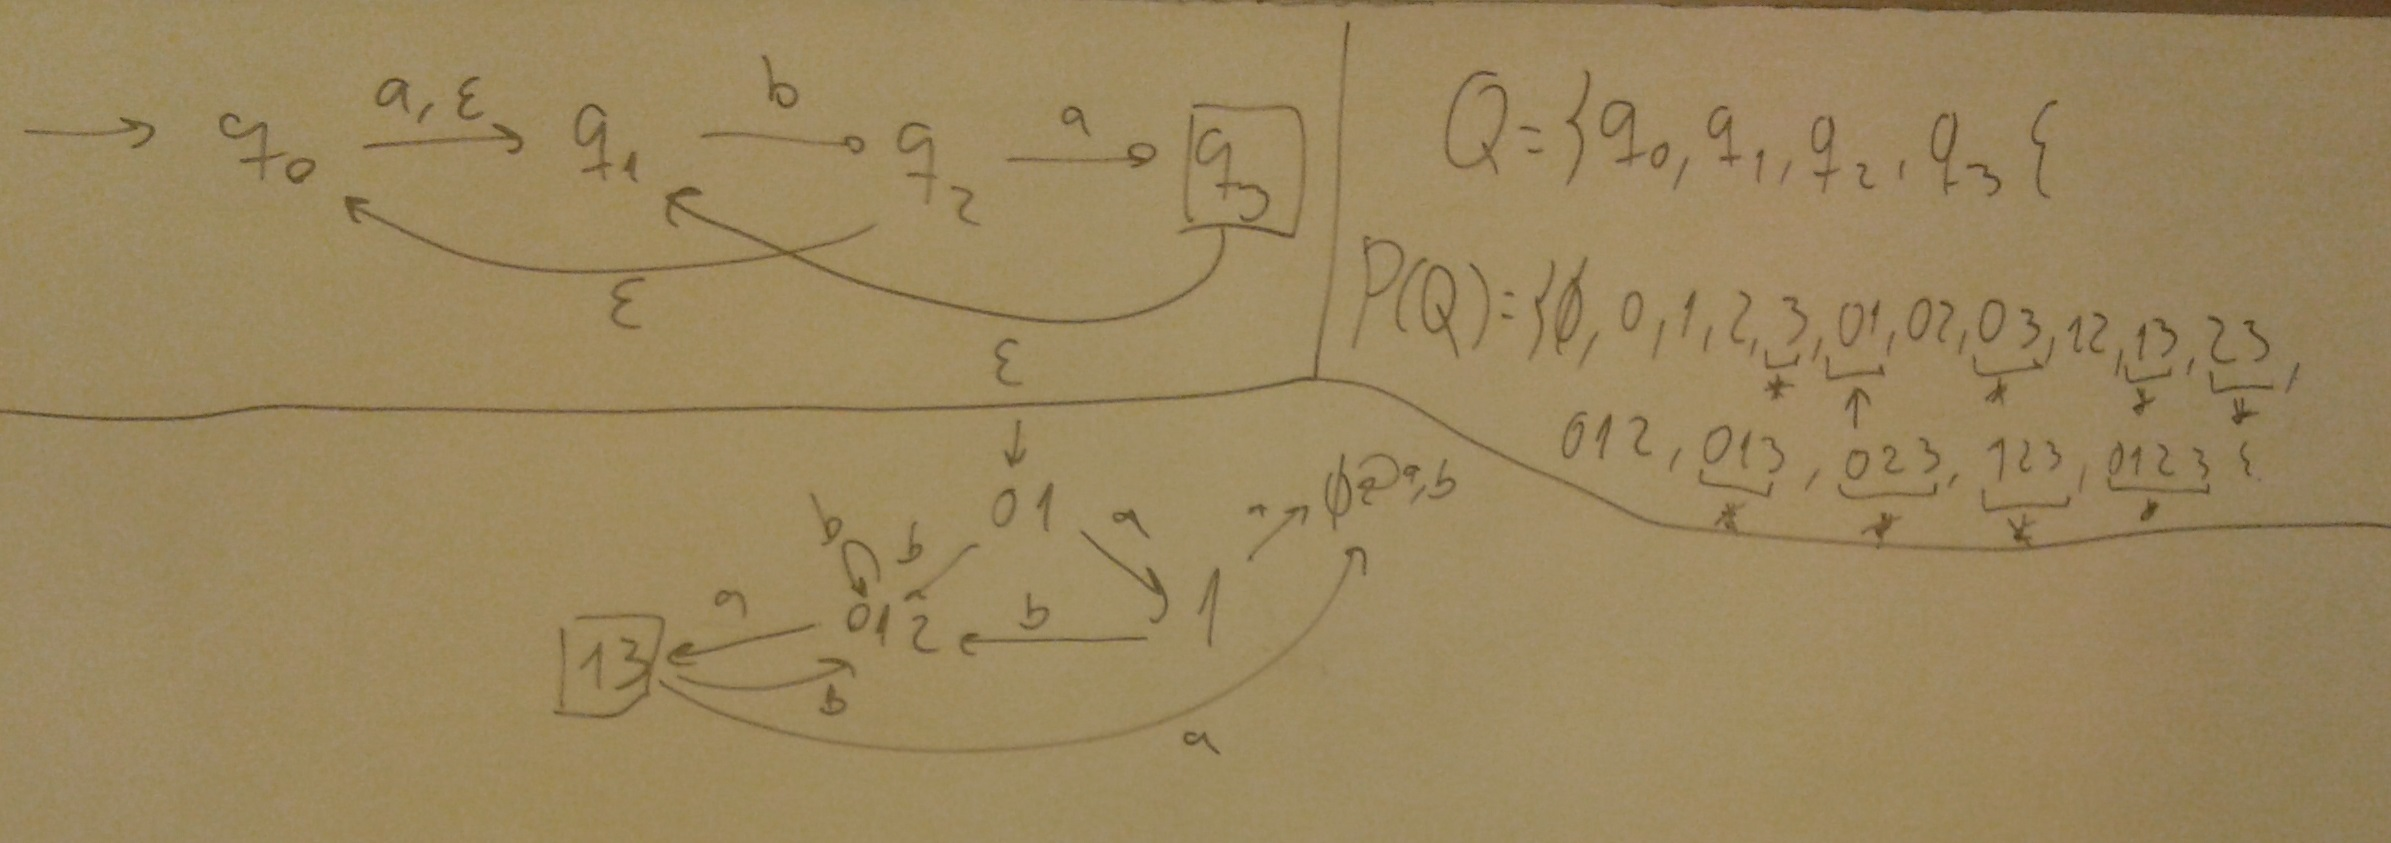
\includegraphics[scale=0.2]{Automatas/12}
\end{figure}\
\end{solucion}

\newpage

\begin{ejercicio}{13}
Consideremos la gramática regular:
\begin{align*}
&S \rightarrow xN\\
&S \rightarrow x\\
&N \rightarrow yM\\
&N \rightarrow y\\
&M \rightarrow zN\\
&M \rightarrow z
\end{align*}
donde $S$ es el símbolo inicial, $\{x, y, z\}$ son terminales y $\{S,N,M\}$ variables. Se pide:
\begin{enumerate}
\item Construir un $\varepsilon$-AFND que acepte el lenguaje generado por $\Gamma$.
\item Encontrar una expresión regular que genere el lenguaje generado por $\Gamma$.
\end{enumerate}
\end{ejercicio}
\begin{solucion}
Tenemos que la siguiente $ϵ$-AFND acepta el lenguaje generado por $Γ$:
\[ 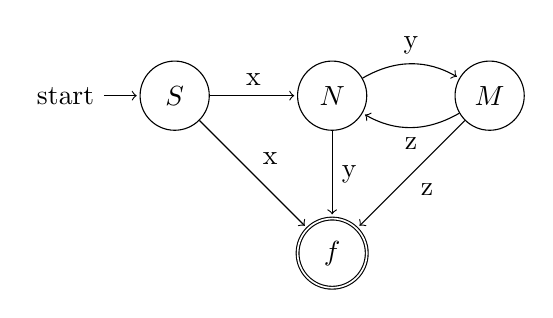
\begin{tikzpicture}[shorten >=1pt,node distance=2cm,on grid,auto]
   \node[state,initial] (S)  {$S$};
   \node[state] (N) [right=of S] {$N$};
   \node[state] (M) [right=of N] {$M$};
   \node[state,accepting] (f) [below=of N] {$f$};
    \path[->]
    (S) edge node {x} (N)
        edge node {x} (f)
    (N) edge [bend left] node {y} (M)
        edge node {y} (f)
    (M) edge [bend left] node {z} (N)
        edge node {z} (f);
\end{tikzpicture} \]

Para encontrar la expresión regular del lenguaje, tomemos primero el AFNDG que acepta el lenguaje:

\[ \begin{tikzpicture}[shorten >=1pt,node distance=2cm,on grid,auto]
   \node[state,initial] (q_I)  {$q_I$};
   \node[state] (S) [right=of q_I] {$S$};
   \node[state] (N) [right=of S] {$N$};
   \node[state] (M) [right=of N] {$M$};
   \node[state] (f) [below=of N] {$f$};
   \node[state,accepting] (q_A) [right=of f] {$q_A$};
    \path[->]
    (q_I) edge node {ϵ} (S)
    (S) edge node {x} (N)
        edge node {x} (f)
    (N) edge [bend left] node {y} (M)
        edge node {y} (f)
    (M) edge [bend left] node {z} (N)
        edge node {z} (f)
    (f) edge node {ϵ} (q_A);
\end{tikzpicture} \]
y vamos eliminando estados:
\[ \begin{tikzpicture}[shorten >=1pt,node distance=2cm,on grid,auto]
   \node[state,initial] (q_I)  {$q_I$};
   \node[state] (S) [right=of q_I] {$S$};
   \node[state] (N) [right=of S] {$N$};
   \node[state] (f) [below=of N] {$f$};
   \node[state,accepting] (q_A) [right=of f] {$q_A$};
    \path[->]
    (q_I) edge node {ϵ} (S)
    (S) edge node {x} (N)
        edge [bend right] node [below] {x} (f)
    (N) edge node {yz+y} (f)
        edge [loop right] node {yz} ()
    (f) edge node {ϵ} (q_A);
\end{tikzpicture} \]
\[ \begin{tikzpicture}[shorten >=1pt,node distance=4cm,on grid,auto]
   \node[state,initial] (q_I)  {$q_I$};
   \node[state] (S) [right=of q_I] {$S$};
   \node[state] (f) [right=of S] {$f$};
   \node[state,accepting] (q_A) [right=of f] {$q_A$};
    \path[->]
    (q_I) edge node {$ϵ$} (S)
    (S) edge node {$x(yz)^*(yz+y)+x$} (f)
    (f) edge node {$ϵ$} (q_A);
\end{tikzpicture} \]
\[ 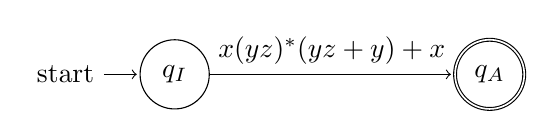
\begin{tikzpicture}[shorten >=1pt,node distance=4cm,on grid,auto]
   \node[state,initial] (q_I)  {$q_I$};
   \node[state,accepting] (q_A) [right=of q_I] {$q_A$};
    \path[->]
    (q_I) edge node {$x(yz)^*(yz+y)+x$} (q_A);
\end{tikzpicture} \]
Al final obtenemos la expresión regular $x(yz)^*(yz+y)+x$.
\end{solucion}

\newpage

\begin{ejercicio}{14}
La siguiente gramática genera el lenguaje $\underline{0}^*\underline{1}(\underline{0} + \underline{1})^*$:
\begin{align*}
&S \rightarrow A1B\\
&A \rightarrow 0A\\
&A \rightarrow \varepsilon\\
&B \rightarrow \varepsilon\\
&B \rightarrow 0B\\
&B \rightarrow 1B\\
\end{align*}
siendo $\{S, A,B\}$ variables, $\{0, 1\}$ terminales y $S$ el símbolo inicial. Obtener derivaciones de las siguientes
palabras:
$$00101,\quad 1001,\quad 00011$$
\end{ejercicio}
\begin{solucion}
$$
S \rightarrow A1B \rightarrow 0A1B \rightarrow 00A1B \rightarrow 001B \rightarrow 0010B \rightarrow 00101B \rightarrow 00101
$$
$$
S \rightarrow A1B \rightarrow 1B\rightarrow 10B\rightarrow 100B\rightarrow 1001B\rightarrow 1001
$$
$$
S \rightarrow A1B \rightarrow 0A1B\rightarrow 00A1B\rightarrow 000A1B\rightarrow 0001B\rightarrow 00011B\rightarrow 00011
$$
\end{solucion}

\newpage

\begin{ejercicio}{15}
Sea $G$ la gramática regular que tiene como producciones:
$$\{S \rightarrow abA, S \rightarrow B, S \rightarrow baB, S \rightarrow \varepsilon, A \rightarrow bS, B \rightarrow aS, A \rightarrow b\}$$
siendo $S$ el símbolo inicial, $a, b$ terminales y $A,B$ variables. Construir un $\varepsilon$-AFND que acepte el
lenguaje generado por $G$.
\end{ejercicio}
\begin{solucion}
Desarrollemos un poco el árbol de derivación de $G$:
\[
\begin{tikzpicture}
  \node {S}
    child { node {abA} 
      child { node {abbS} } 
      child { node {abb} } }
    child { node {B} 
      child { node {aS} } }
    child { node {baB} 
      child { node {baaS} } }
    child { node {ϵ} };
\end{tikzpicture}
\]
Entonces $G$ genera el lenguage $(a+abb+baa)^*$. Construimos un $ϵ$-AFND que acepte este lenguaje:
\[
\begin{tikzpicture}[shorten >=1pt,node distance=2cm,on grid,auto] 
   \node[state,initial,accepting] (q_0)   {$q_0$}; 
   \node[state] (q_1) [above right=of q_0] {$q_1$};
   \node[state] (q_2) [below right=of q_0] {$q_2$};
   \node[state] (q_3) [right=of q_1] {$q_3$};
   \node[state] (q_4) [right=of q_2] {$q_4$};
    \path[->] 
    (q_0) edge node [below] {a} (q_1)
          edge node [below left] {b} (q_2)
    (q_1) edge [bend right] node [above] {ϵ} (q_0)
          edge node {b} (q_3)
    (q_3) edge node {b} (q_0)
    (q_2) edge node [below] {a} (q_4)
    (q_4) edge node [above] {a} (q_0);
\end{tikzpicture}
\]
\end{solucion}

\newpage

\begin{ejercicio}{16}
Describir una gramática regular que genere el lenguaje aceptado por el siguiente
autómata:
\[
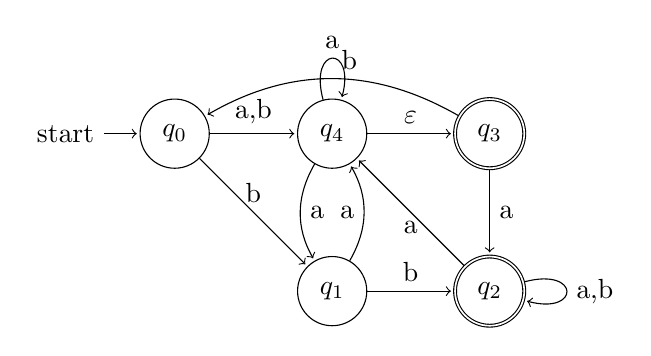
\begin{tikzpicture}[shorten >=1pt,node distance=2cm,on grid,auto] 
   \node[state,initial] (q_0)   {$q_0$}; 
   \node[state] (q_4) [right=of q_0] {$q_4$};
   \node[state] (q_1) [below =of q_4] {$q_1$};
   \node[state, accepting] (q_3) [right=of q_4] {$q_3$};
   \node[state, accepting] (q_2) [below=of q_3] {$q_2$};
    \path[->] 
    (q_0) edge node [above] {b} (q_1)
          edge node [above] {a,b} (q_4)
    (q_1) edge node [above] {b} (q_2)
    	  edge [bend right] node [left] {a} (q_4)
    (q_3) edge node {a} (q_2)
    	  edge [bend right] node [above right] {b} (q_0)
    (q_2) edge node [below] {a} (q_4)
    	  edge [loop right] node {a,b} (q_2)
    (q_4) edge node [above] {$\varepsilon$} (q_3)
          edge [loop above] node {a} (q_4)
     	  edge [bend right] node [right] {a} (q_1);
\end{tikzpicture}
\]
\end{ejercicio}
\begin{solucion}
Definimos el conjunto de variables $\{S, V_1, V_2, V_3,V_4\}$ y los terminales $\{a,b\}$.
Entonces la gramática queda determinada por las siguientes reglas de producción:
\begin{align*}
&S\to aV_4 & S\to b V_4 & & S\to b V_1\\
&V_1\to aV_4 & V_1\to b V_2 \\
&V_2\to aV_2 & V_2\to bV_2 & & V_2\to aV_4& &V_2\to \varepsilon\\
& V_3\to bS & V_3\to aV_2 & &V_3\to \varepsilon\\
& V_4\to V_3 & V_4\to aV_1 & &V_4\to a V_4
\end{align*}
\end{solucion}

\newpage

\begin{ejercicio}{17}
Probar que los siguientes lenguajes sobre el alfabeto $Σ = \{0, 1\}$ no son regulares:
\begin{itemize}
\item $L = \{x ∈ Σ^*
: x$ contiene el mismo número de 0’s y de 1’s$\}$.

\item $L = \{x ∈ Σ^*
: |x|$ es primo$\}$.
\item $L = \{0^p
: p$ primo$\}$.
\item $L = \{0^n1^m : n \neq m\}$.
\item $L = \{0^n1^{2n}
: n \neq 0\}$.
\item $L = \{0^n1^m : 0 < n ≤ m\}$.
\end{itemize}
\end{ejercicio}
\begin{solucion}\mbox{}
\begin{itemize}
	\item Supongamos que $L$ fuera regular. Sea $M$ una AFD tal que $L(M)=L$ y $n$ el número de estados en $M$. Sea $x \in L$ tal que $x=0\dots01\dots1$ de longitud $2n$. Por el lema del bombeo, existen $u$, $v$ y $w$ en $\{0,1\}^*$ tal que $x=uvw$, $v \neq ϵ$, $|uv|≤n$ y $uv^kw \in L$ para todo $k \in \N$. Como $|uv|≤n$, $v$ tiene $m$ $0$'s con $m ≤ n$. Tomando $k=n$, tenemos que $uv^nw \in L$. Sin embargo, $v^n$ tiene $n\cdot m$ $0$'s, mientras $w$ tiene como mucho $n$ $1$'s. Contradicción.
	\item Supongamos que $L$ fuera regular. Sea $M$ una AFD tal que $L(M)=L$ y $n$ el número de estados en $M$. Sea $x=0\dots0\in L$ de longitud $p$ con $p > n+1$. Aplicamos el lema del bombeo para descomponer $x=uvw$. Como $|uv| ≤ n < p$, $|w|≥2$. Tenemos que $uv^kw \in L$ para todo $k \in \N$. Sin embargo, $|uv^{|uw|}w|=|uw|+|v||uw|$, que es divisible por $|uw|>1$, luego no es primo. Contradicción.
	\item Véase el apartado anterior.
	\item Supongamos que $L$ fuera regular. Sea $M$ una AFD tal que $L(M)=L$ y $n$ el número de estados en $M$. Sea $x=0^n1^{n+n!}\in L$. Aplicamos el lema del bombeo para descomponer $x=uvw$. Como $|uv|≤n$, $v=0^m$ con $m≤n$. Sea $w=0^a1^b$. Consideramos la palabra $uv^{1+n!/m}w$. Su número de $0$'s es $n+\frac{n!}{m}\cdot m=n+n!$, que es el mismo su número de $1$'s, luego $uv^{n!/m}w \notin L$. Contradicción.
	\item Supongamos que $L$ fuera regular. Sea $M$ una AFD tal que $L(M)=L$ y $n$ el número de estados en $M$. Tomamos $x=0^{n}1^{2n}$. Aplicamos el lema del bombeo para descomponer $x=uvw$. Como $|uv|≤n$, $v=0^m$ con $1≤m≤n$. Consideramos la palabra $uv^2w=0^{n+m}1^{2n}$. Como $m \neq 0$, llegamos a que $uv^2w \notin L$. Contradicción.
	\item Supongamos que $L$ fuera regular. Sea $M$ una AFD tal que $L(M)=L$ y $n$ el número de estados en $M$. Tomamos $x=0^n1^n$. Aplicamos el lema del bombeo para descomponer $x=uvw$. Como $|uv|≤n$, $v=0^m$ con $1≤m≤n$. Basta observar entonces que $uv^2w$ tiene $n+m$ $0$'s y $n$ $1$'s, luego $uv^2w \notin L$. Contradicción.
\end{itemize}
\end{solucion}

\newpage

\begin{ejercicio}{18}
Sean $L_1$ y $L_2$ dos lenguajes sobre un alfabeto $Σ$. Definimos el cociente por la derecha
de $L_1$ y $L_2$ como el lenguaje:
$$L_1/L_2 = \{x ∈ Σ^*
: \text{ existe } y ∈ L_2\text{ tal que }xy ∈ L_1\}.$$
Probar que si $L_1$ y $L_2$ son regulares entonces $L_1/L_2$ también es regular.
\end{ejercicio}
\begin{solucion}
Consideramos el AFD $M=(Q,Σ,δ,q_0,F)$ tal que $L(M)=L_1$. Definimos una AFD $M'=(Q,Σ,δ,q_0,F')$, idéntica a $M$ excepto por los estados finales $F'$ que definimos como:
\[ F' = \{q \in Q \mid \exists y \in L_2 \text{ tal que }\hat{δ}(q,y) \in F \}\]
El lenguaje aceptado por $M'$ es:
\begin{align*}
	L(M') & = \{x \in Σ^* : \hat{δ}(q_0,x) \in F'\} = \{x \in Σ^* : \exists y \in L_2 \text{ tal que } \hat{δ}(\hat{δ}(q_0,x),y) \in F\} =\\
	& = \{x \in Σ^* : \exists y \in L_2 \text{ tal que } \hat{δ}(q_0,xy) \in F\} = \{x \in Σ^* : \exists y \in L_2 \text{ tal que } xy \in L_1\}=\\
	& = L_1/L_2
\end{align*}
Obsérvese que no ha sido necesaria la hipótesis de que $L_2$ sea regular.
\end{solucion}

\newpage

\begin{ejercicio}{19}
Probar que el lenguaje sobre el alfabeto $Σ = \{a, b\}$,
$$L = \{a^pb^m : p \text{ es primo y }m > 0\} + \{a^n
: n ≥ 0\}$$
no es regular.
\end{ejercicio}
\begin{solucion}
Supongamos que el lenguaje es regular y su autómata tiene $n$ estados. Sea $x=a^pb^m$ con $p\geq n$ y $m\geq 1$. Entonces por el lema del bombeo tenemos una descomposición $x=uvw$ con $v\neq\varepsilon$ y $|uv|\leq n$. Entonces $v=a^s$ para algún $1\leq s\leq n\leq p$. Así que $u=a^l$ para algún $0\leq l\leq n-s$. Además, $w=a^tb^m$ con $t=n-s-l$. Entonces, por el lema tendríamos que $uv^kw\in L\ \forall k\in\N$, lo cual es equivalente a decir que $a^la^{ks}a^tb^m\in L\ \forall k\in\N$. Entonces basta elegir $k$ de modo que $l+ks+t$ no sea primo para llegar a una contradicción.
\end{solucion}


\end{document}